\documentclass[runningheads]{llncs}
\usepackage[T1]{fontenc}
\usepackage{graphicx}
\usepackage{amsmath,amssymb}
\usepackage{booktabs}
\usepackage{algorithm}
\usepackage[noend]{algpseudocode}
\usepackage[section]{placeins}
\usepackage{url}
\usepackage{hyperref}
\hypersetup{colorlinks=true,linkcolor=blue,citecolor=blue,urlcolor=blue}
\renewcommand\UrlFont{\color{blue}\rmfamily}
% float placement: allow up to two floats on a text page and fill float pages
\renewcommand{\topfraction}{0.9}
\renewcommand{\bottomfraction}{0.6}
\renewcommand{\textfraction}{0.08}
\renewcommand{\floatpagefraction}{0.85}
\setcounter{topnumber}{2}
\setcounter{totalnumber}{3}

% every number in the text is generated from the result files (scripts/build_numbers.py)
% generated by scripts/build_numbers.py -- do not edit
\expandafter\def\csname data@bench_cpu_assoc_128_C1_ms\endcsname{6575}
\expandafter\def\csname data@bench_cpu_assoc_128_C2_ms\endcsname{5739}
\expandafter\def\csname data@bench_cpu_assoc_128_C2s_ms\endcsname{6767}
\expandafter\def\csname data@bench_cpu_assoc_128_E0_ms\endcsname{3580}
\expandafter\def\csname data@bench_cpu_assoc_128_E1_ms\endcsname{4702}
\expandafter\def\csname data@bench_cpu_assoc_128_E2_ms\endcsname{3477}
\expandafter\def\csname data@bench_cpu_assoc_128_P1_ms\endcsname{nan}
\expandafter\def\csname data@bench_cpu_assoc_32_C1_ms\endcsname{3425}
\expandafter\def\csname data@bench_cpu_assoc_32_C2_ms\endcsname{2914}
\expandafter\def\csname data@bench_cpu_assoc_32_C2s_ms\endcsname{2926}
\expandafter\def\csname data@bench_cpu_assoc_32_E0_ms\endcsname{739}
\expandafter\def\csname data@bench_cpu_assoc_32_E1_ms\endcsname{1801}
\expandafter\def\csname data@bench_cpu_assoc_32_E2_ms\endcsname{1706}
\expandafter\def\csname data@bench_cpu_assoc_32_P1_ms\endcsname{nan}
\expandafter\def\csname data@bench_cpu_l1_128_C1_ms\endcsname{3550}
\expandafter\def\csname data@bench_cpu_l1_128_C2_ms\endcsname{5011}
\expandafter\def\csname data@bench_cpu_l1_128_C2s_ms\endcsname{6533}
\expandafter\def\csname data@bench_cpu_l1_128_E0_ms\endcsname{387}
\expandafter\def\csname data@bench_cpu_l1_128_E1_ms\endcsname{1485}
\expandafter\def\csname data@bench_cpu_l1_128_E2_ms\endcsname{3250}
\expandafter\def\csname data@bench_cpu_l1_128_P1_ms\endcsname{nan}
\expandafter\def\csname data@bench_cpu_l1_32_C1_ms\endcsname{1377}
\expandafter\def\csname data@bench_cpu_l1_32_C2_ms\endcsname{2193}
\expandafter\def\csname data@bench_cpu_l1_32_C2s_ms\endcsname{2523}
\expandafter\def\csname data@bench_cpu_l1_32_E0_ms\endcsname{98}
\expandafter\def\csname data@bench_cpu_l1_32_E1_ms\endcsname{568}
\expandafter\def\csname data@bench_cpu_l1_32_E2_ms\endcsname{1595}
\expandafter\def\csname data@bench_cpu_l1_32_P1_ms\endcsname{nan}
\expandafter\def\csname data@bench_gpu_assoc_128_C1_mb\endcsname{4025}
\expandafter\def\csname data@bench_gpu_assoc_128_C1_ms\endcsname{185}
\expandafter\def\csname data@bench_gpu_assoc_128_C2_mb\endcsname{4435}
\expandafter\def\csname data@bench_gpu_assoc_128_C2_ms\endcsname{152}
\expandafter\def\csname data@bench_gpu_assoc_128_C2s_mb\endcsname{5808}
\expandafter\def\csname data@bench_gpu_assoc_128_C2s_ms\endcsname{211}
\expandafter\def\csname data@bench_gpu_assoc_128_E0_mb\endcsname{6949}
\expandafter\def\csname data@bench_gpu_assoc_128_E0_ms\endcsname{250}
\expandafter\def\csname data@bench_gpu_assoc_128_E1_mb\endcsname{1078}
\expandafter\def\csname data@bench_gpu_assoc_128_E1_ms\endcsname{77}
\expandafter\def\csname data@bench_gpu_assoc_128_E2_mb\endcsname{1606}
\expandafter\def\csname data@bench_gpu_assoc_128_E2_ms\endcsname{103}
\expandafter\def\csname data@bench_gpu_assoc_128_P1_mb\endcsname{21255}
\expandafter\def\csname data@bench_gpu_assoc_128_P1_ms\endcsname{372}
\expandafter\def\csname data@bench_gpu_assoc_32_C1_mb\endcsname{1283}
\expandafter\def\csname data@bench_gpu_assoc_32_C1_ms\endcsname{164}
\expandafter\def\csname data@bench_gpu_assoc_32_C2_mb\endcsname{1796}
\expandafter\def\csname data@bench_gpu_assoc_32_C2_ms\endcsname{134}
\expandafter\def\csname data@bench_gpu_assoc_32_C2s_mb\endcsname{2152}
\expandafter\def\csname data@bench_gpu_assoc_32_C2s_ms\endcsname{108}
\expandafter\def\csname data@bench_gpu_assoc_32_E0_mb\endcsname{1767}
\expandafter\def\csname data@bench_gpu_assoc_32_E0_ms\endcsname{74}
\expandafter\def\csname data@bench_gpu_assoc_32_E1_mb\endcsname{516}
\expandafter\def\csname data@bench_gpu_assoc_32_E1_ms\endcsname{58}
\expandafter\def\csname data@bench_gpu_assoc_32_E2_mb\endcsname{1058}
\expandafter\def\csname data@bench_gpu_assoc_32_E2_ms\endcsname{47}
\expandafter\def\csname data@bench_gpu_assoc_32_P1_mb\endcsname{5350}
\expandafter\def\csname data@bench_gpu_assoc_32_P1_ms\endcsname{101}
\expandafter\def\csname data@bench_gpu_assoc_512_C1_mb\endcsname{15041}
\expandafter\def\csname data@bench_gpu_assoc_512_C1_ms\endcsname{360}
\expandafter\def\csname data@bench_gpu_assoc_512_C2_mb\endcsname{15361}
\expandafter\def\csname data@bench_gpu_assoc_512_C2_ms\endcsname{487}
\expandafter\def\csname data@bench_gpu_assoc_512_C2s_mb\endcsname{21261}
\expandafter\def\csname data@bench_gpu_assoc_512_C2s_ms\endcsname{766}
\expandafter\def\csname data@bench_gpu_assoc_512_E0_mb\endcsname{27689}
\expandafter\def\csname data@bench_gpu_assoc_512_E0_ms\endcsname{960}
\expandafter\def\csname data@bench_gpu_assoc_512_E1_mb\endcsname{3338}
\expandafter\def\csname data@bench_gpu_assoc_512_E1_ms\endcsname{208}
\expandafter\def\csname data@bench_gpu_assoc_512_E2_mb\endcsname{3803}
\expandafter\def\csname data@bench_gpu_assoc_512_E2_ms\endcsname{346}
\expandafter\def\csname data@bench_gpu_assoc_512_P1_mb\endcsname{nan}
\expandafter\def\csname data@bench_gpu_assoc_512_P1_ms\endcsname{nan}
\expandafter\def\csname data@bench_gpu_l1_128_C1_mb\endcsname{4001}
\expandafter\def\csname data@bench_gpu_l1_128_C1_ms\endcsname{179}
\expandafter\def\csname data@bench_gpu_l1_128_C2_mb\endcsname{4422}
\expandafter\def\csname data@bench_gpu_l1_128_C2_ms\endcsname{150}
\expandafter\def\csname data@bench_gpu_l1_128_C2s_mb\endcsname{5795}
\expandafter\def\csname data@bench_gpu_l1_128_C2s_ms\endcsname{210}
\expandafter\def\csname data@bench_gpu_l1_128_E0_mb\endcsname{942}
\expandafter\def\csname data@bench_gpu_l1_128_E0_ms\endcsname{37}
\expandafter\def\csname data@bench_gpu_l1_128_E1_mb\endcsname{1054}
\expandafter\def\csname data@bench_gpu_l1_128_E1_ms\endcsname{72}
\expandafter\def\csname data@bench_gpu_l1_128_E2_mb\endcsname{1592}
\expandafter\def\csname data@bench_gpu_l1_128_E2_ms\endcsname{104}
\expandafter\def\csname data@bench_gpu_l1_128_P1_mb\endcsname{1038}
\expandafter\def\csname data@bench_gpu_l1_128_P1_ms\endcsname{28}
\expandafter\def\csname data@bench_gpu_l1_32_C1_mb\endcsname{1251}
\expandafter\def\csname data@bench_gpu_l1_32_C1_ms\endcsname{155}
\expandafter\def\csname data@bench_gpu_l1_32_C2_mb\endcsname{1775}
\expandafter\def\csname data@bench_gpu_l1_32_C2_ms\endcsname{130}
\expandafter\def\csname data@bench_gpu_l1_32_C2s_mb\endcsname{2127}
\expandafter\def\csname data@bench_gpu_l1_32_C2s_ms\endcsname{109}
\expandafter\def\csname data@bench_gpu_l1_32_E0_mb\endcsname{236}
\expandafter\def\csname data@bench_gpu_l1_32_E0_ms\endcsname{35}
\expandafter\def\csname data@bench_gpu_l1_32_E1_mb\endcsname{482}
\expandafter\def\csname data@bench_gpu_l1_32_E1_ms\endcsname{53}
\expandafter\def\csname data@bench_gpu_l1_32_E2_mb\endcsname{1044}
\expandafter\def\csname data@bench_gpu_l1_32_E2_ms\endcsname{46}
\expandafter\def\csname data@bench_gpu_l1_32_P1_mb\endcsname{273}
\expandafter\def\csname data@bench_gpu_l1_32_P1_ms\endcsname{30}
\expandafter\def\csname data@bench_gpu_l1_512_C1_mb\endcsname{15018}
\expandafter\def\csname data@bench_gpu_l1_512_C1_ms\endcsname{305}
\expandafter\def\csname data@bench_gpu_l1_512_C2_mb\endcsname{15348}
\expandafter\def\csname data@bench_gpu_l1_512_C2_ms\endcsname{486}
\expandafter\def\csname data@bench_gpu_l1_512_C2s_mb\endcsname{21248}
\expandafter\def\csname data@bench_gpu_l1_512_C2s_ms\endcsname{765}
\expandafter\def\csname data@bench_gpu_l1_512_E0_mb\endcsname{3708}
\expandafter\def\csname data@bench_gpu_l1_512_E0_ms\endcsname{73}
\expandafter\def\csname data@bench_gpu_l1_512_E1_mb\endcsname{3315}
\expandafter\def\csname data@bench_gpu_l1_512_E1_ms\endcsname{151}
\expandafter\def\csname data@bench_gpu_l1_512_E2_mb\endcsname{3791}
\expandafter\def\csname data@bench_gpu_l1_512_E2_ms\endcsname{346}
\expandafter\def\csname data@bench_gpu_l1_512_P1_mb\endcsname{4055}
\expandafter\def\csname data@bench_gpu_l1_512_P1_ms\endcsname{70}
\expandafter\def\csname data@binom_p_max\endcsname{$4\times10^{-8}$}
\expandafter\def\csname data@cheb_err_r16\endcsname{$2.7\times10^{-3}$}
\expandafter\def\csname data@cheb_err_r32\endcsname{$1.9\times10^{-4}$}
\expandafter\def\csname data@cheb_err_r4\endcsname{$1.3\times10^{-1}$}
\expandafter\def\csname data@cheb_err_r8\endcsname{$6.0\times10^{-2}$}
\expandafter\def\csname data@eq_cheb16_dense_dd\endcsname{$2.4\times10^{-5}$}
\expandafter\def\csname data@eq_cheb16_dense_dx\endcsname{$3.5\times10^{-5}$}
\expandafter\def\csname data@eq_cheb16_spmm_dd\endcsname{$2.4\times10^{-5}$}
\expandafter\def\csname data@eq_cheb16_spmm_dx\endcsname{$3.5\times10^{-5}$}
\expandafter\def\csname data@eq_cheb32_dense_dd\endcsname{$2.4\times10^{-5}$}
\expandafter\def\csname data@eq_cheb32_dense_dx\endcsname{$3.5\times10^{-5}$}
\expandafter\def\csname data@eq_cheb32_spmm_dd\endcsname{$2.4\times10^{-5}$}
\expandafter\def\csname data@eq_cheb32_spmm_dx\endcsname{$3.5\times10^{-5}$}
\expandafter\def\csname data@eq_cheb4_dense_dd\endcsname{$2.1\times10^{-3}$}
\expandafter\def\csname data@eq_cheb4_dense_dx\endcsname{$3.0\times10^{-3}$}
\expandafter\def\csname data@eq_cheb4_spmm_dd\endcsname{$2.1\times10^{-3}$}
\expandafter\def\csname data@eq_cheb4_spmm_dx\endcsname{$3.0\times10^{-3}$}
\expandafter\def\csname data@eq_cheb8_dense_dd\endcsname{$3.6\times10^{-4}$}
\expandafter\def\csname data@eq_cheb8_dense_dx\endcsname{$5.2\times10^{-4}$}
\expandafter\def\csname data@eq_cheb8_spmm_dd\endcsname{$3.6\times10^{-4}$}
\expandafter\def\csname data@eq_cheb8_spmm_dx\endcsname{$5.2\times10^{-4}$}
\expandafter\def\csname data@eq_scale\endcsname{0.087}
\expandafter\def\csname data@fallback_gain_max\endcsname{0.002}
\expandafter\def\csname data@g7_base_L2_HepG2_rc\endcsname{0.232}
\expandafter\def\csname data@g7_base_L2_HepG2_rr\endcsname{0.206}
\expandafter\def\csname data@g7_base_L2_Jurkat_rc\endcsname{0.234}
\expandafter\def\csname data@g7_base_L2_Jurkat_rr\endcsname{0.218}
\expandafter\def\csname data@g7_base_L2_K562_rc\endcsname{0.227}
\expandafter\def\csname data@g7_base_L2_K562_rewired_rc\endcsname{0.163}
\expandafter\def\csname data@g7_base_L2_K562_rewired_rr\endcsname{0.138}
\expandafter\def\csname data@g7_base_L2_K562_rr\endcsname{0.203}
\expandafter\def\csname data@g7_base_rc\endcsname{0.238}
\expandafter\def\csname data@g7_base_rr\endcsname{0.221}
\expandafter\def\csname data@g7_d_k_base\endcsname{-0.011 [-0.019, -0.004]}
\expandafter\def\csname data@g7_d_k_hep\endcsname{-0.005 [-0.011, 0.000]}
\expandafter\def\csname data@g7_d_k_jur\endcsname{-0.008 [-0.015, 0.000]}
\expandafter\def\csname data@g7_d_k_rew\endcsname{+0.064 [+0.052, +0.076]}
\expandafter\def\csname data@g7c_jaccard_HepG2_Jurkat\endcsname{0.05}
\expandafter\def\csname data@g7c_jaccard_HepG2_K562\endcsname{0.08}
\expandafter\def\csname data@g7c_jaccard_Jurkat_K562\endcsname{0.07}
\expandafter\def\csname data@g7c_n_edges_HepG2\endcsname{335,734}
\expandafter\def\csname data@g7c_n_edges_Jurkat\endcsname{80,414}
\expandafter\def\csname data@g7c_n_edges_K562\endcsname{645,570}
\expandafter\def\csname data@g7c_tf_outdeg_spearman_HepG2_Jurkat\endcsname{0.58}
\expandafter\def\csname data@g7c_tf_outdeg_spearman_HepG2_K562\endcsname{0.31}
\expandafter\def\csname data@g7c_tf_outdeg_spearman_Jurkat_K562\endcsname{0.71}
\expandafter\def\csname data@k562_b0_ap\endcsname{0.099}
\expandafter\def\csname data@k562_b0_cent\endcsname{0.503}
\expandafter\def\csname data@k562_b0_r20\endcsname{0.116}
\expandafter\def\csname data@k562_b0_rc\endcsname{0.096}
\expandafter\def\csname data@k562_b0_rr\endcsname{0.000}
\expandafter\def\csname data@k562_b1_raw\endcsname{0.26}
\expandafter\def\csname data@k562_b2_ap\endcsname{0.110}
\expandafter\def\csname data@k562_b2_cent\endcsname{0.641}
\expandafter\def\csname data@k562_b2_r20\endcsname{0.275}
\expandafter\def\csname data@k562_b2_rc\endcsname{0.145}
\expandafter\def\csname data@k562_b2_rr\endcsname{0.139}
\expandafter\def\csname data@k562_binom_p\endcsname{$2\times10^{-10}$}
\expandafter\def\csname data@k562_cfg\endcsname{fold 0: $k$=40, $\alpha$=0.75; fold 1: $k$=40, $\alpha$=0.75; fold 2: $k$=40, $\alpha$=0.75}
\expandafter\def\csname data@k562_concord\endcsname{80}
\expandafter\def\csname data@k562_d_gcn_ip_rc\endcsname{+0.029 [+0.019, +0.038]}
\expandafter\def\csname data@k562_d_gcn_ip_rr\endcsname{+0.019 [+0.011, +0.027]}
\expandafter\def\csname data@k562_d_gcn_rew_rc\endcsname{+0.123 [+0.107, +0.139]}
\expandafter\def\csname data@k562_d_gcn_rew_rr\endcsname{+0.117 [+0.104, +0.131]}
\expandafter\def\csname data@k562_d_ip_b2_rc\endcsname{+0.093 [+0.077, +0.108]}
\expandafter\def\csname data@k562_d_ip_b2_rr\endcsname{+0.083 [+0.069, +0.097]}
\expandafter\def\csname data@k562_d_ip_knn_rc\endcsname{+0.091 [+0.076, +0.107]}
\expandafter\def\csname data@k562_d_ip_knn_rr\endcsname{+0.081 [+0.067, +0.095]}
\expandafter\def\csname data@k562_d_ip_noself_rc\endcsname{+0.098 [+0.084, +0.113]}
\expandafter\def\csname data@k562_d_ip_noself_rr\endcsname{+0.086 [+0.073, +0.100]}
\expandafter\def\csname data@k562_d_ip_rew_rc\endcsname{+0.097 [+0.081, +0.113]}
\expandafter\def\csname data@k562_d_ip_rew_rr\endcsname{+0.087 [+0.073, +0.102]}
\expandafter\def\csname data@k562_d_ip_str_l1_rc\endcsname{+0.003 [-0.001, +0.007]}
\expandafter\def\csname data@k562_d_ip_str_l1_rr\endcsname{-0.001 [-0.003, +0.001]}
\expandafter\def\csname data@k562_d_nbr_ip_rc\endcsname{+0.047 [+0.035, +0.060]}
\expandafter\def\csname data@k562_d_nbr_ip_rr\endcsname{+0.054 [+0.045, +0.064]}
\expandafter\def\csname data@k562_faith1\endcsname{0.000 [-0.002, +0.003]}
\expandafter\def\csname data@k562_faith5\endcsname{+0.008 [+0.001, +0.016]}
\expandafter\def\csname data@k562_faith_n\endcsname{651}
\expandafter\def\csname data@k562_g2_b3_b2\endcsname{-0.0013 [-0.0043, +0.0004]}
\expandafter\def\csname data@k562_g2_h2_b2\endcsname{+0.0001 [-0.0003, +0.0007]}
\expandafter\def\csname data@k562_g2_h2_b3\endcsname{+0.0014 [-0.0001, +0.0041]}
\expandafter\def\csname data@k562_g2_h2_rew\endcsname{+0.0001 [-0.0002, +0.0005]}
\expandafter\def\csname data@k562_g2_reach_n\endcsname{37}
\expandafter\def\csname data@k562_g2_reach_pct\endcsname{5.3}
\expandafter\def\csname data@k562_gcn_ap\endcsname{0.140}
\expandafter\def\csname data@k562_gcn_cent\endcsname{0.755}
\expandafter\def\csname data@k562_gcn_r20\endcsname{0.454}
\expandafter\def\csname data@k562_gcn_rc\endcsname{0.267}
\expandafter\def\csname data@k562_gcn_rr\endcsname{0.240}
\expandafter\def\csname data@k562_gcnrew_ap\endcsname{0.106}
\expandafter\def\csname data@k562_gcnrew_cent\endcsname{0.641}
\expandafter\def\csname data@k562_gcnrew_r20\endcsname{0.263}
\expandafter\def\csname data@k562_gcnrew_rc\endcsname{0.144}
\expandafter\def\csname data@k562_gcnrew_rr\endcsname{0.123}
\expandafter\def\csname data@k562_genes\endcsname{8,563}
\expandafter\def\csname data@k562_ip_ap\endcsname{0.132}
\expandafter\def\csname data@k562_ip_cent\endcsname{0.737}
\expandafter\def\csname data@k562_ip_r20\endcsname{0.434}
\expandafter\def\csname data@k562_ip_rc\endcsname{0.238}
\expandafter\def\csname data@k562_ip_rr\endcsname{0.221}
\expandafter\def\csname data@k562_iso_pct\endcsname{1.6}
\expandafter\def\csname data@k562_knn_ap\endcsname{0.112}
\expandafter\def\csname data@k562_knn_cent\endcsname{0.640}
\expandafter\def\csname data@k562_knn_r20\endcsname{0.277}
\expandafter\def\csname data@k562_knn_rc\endcsname{0.147}
\expandafter\def\csname data@k562_knn_rr\endcsname{0.141}
\expandafter\def\csname data@k562_n_tf\endcsname{8}
\expandafter\def\csname data@k562_nbr_ap\endcsname{0.162}
\expandafter\def\csname data@k562_nbr_cent\endcsname{0.791}
\expandafter\def\csname data@k562_nbr_r20\endcsname{0.511}
\expandafter\def\csname data@k562_nbr_rc\endcsname{0.285}
\expandafter\def\csname data@k562_nbr_rr\endcsname{0.276}
\expandafter\def\csname data@k562_nuniq\endcsname{699}
\expandafter\def\csname data@k562_perts\endcsname{2,021}
\expandafter\def\csname data@k562_reach100_pct\endcsname{4.4}
\expandafter\def\csname data@k562_resp_edges\endcsname{109}
\expandafter\def\csname data@k562_rew_ap\endcsname{0.110}
\expandafter\def\csname data@k562_rew_cent\endcsname{0.633}
\expandafter\def\csname data@k562_rew_r20\endcsname{0.268}
\expandafter\def\csname data@k562_rew_rc\endcsname{0.141}
\expandafter\def\csname data@k562_rew_rr\endcsname{0.134}
\expandafter\def\csname data@k562_scc_diff\endcsname{$1\times10^{-13}$}
\expandafter\def\csname data@k562_scc_largest\endcsname{297}
\expandafter\def\csname data@k562_scc_nodes\endcsname{8,563}
\expandafter\def\csname data@k562_scc_reach_only\endcsname{1.4}
\expandafter\def\csname data@k562_scc_speed\endcsname{2.3}
\expandafter\def\csname data@k562_scc_vs_reach\endcsname{1.4}
\expandafter\def\csname data@k562_signed_out_pct\endcsname{5.8}
\expandafter\def\csname data@k562_str_ap\endcsname{0.132}
\expandafter\def\csname data@k562_str_cent\endcsname{0.735}
\expandafter\def\csname data@k562_str_r20\endcsname{0.430}
\expandafter\def\csname data@k562_str_rc\endcsname{0.235}
\expandafter\def\csname data@k562_str_rr\endcsname{0.223}
\expandafter\def\csname data@k562_targets\endcsname{1,835}
\expandafter\def\csname data@k562_tf_wilcoxon_p\endcsname{0.008}
\expandafter\def\csname data@k562_train_edges\endcsname{1,576}
\expandafter\def\csname data@l1_signed\endcsname{61,215}
\expandafter\def\csname data@l1_unique\endcsname{120,312}
\expandafter\def\csname data@memratio_hi\endcsname{8.3}
\expandafter\def\csname data@memratio_lo\endcsname{6.4}
\expandafter\def\csname data@pe_edge_r16_128_gb\endcsname{OOM}
\expandafter\def\csname data@pe_edge_r16_32_gb\endcsname{14.7}
\expandafter\def\csname data@pe_edge_r16_512_gb\endcsname{OOM}
\expandafter\def\csname data@pe_edge_r8_128_gb\endcsname{31.9}
\expandafter\def\csname data@pe_edge_r8_32_gb\endcsname{8.1}
\expandafter\def\csname data@pe_edge_r8_512_gb\endcsname{OOM}
\expandafter\def\csname data@pe_equiv\endcsname{$1\times10^{-7}$}
\expandafter\def\csname data@pe_memratio_r8_128\endcsname{6.2}
\expandafter\def\csname data@pe_spmm_r16_128_gb\endcsname{9.9}
\expandafter\def\csname data@pe_spmm_r16_32_gb\endcsname{6.5}
\expandafter\def\csname data@pe_spmm_r16_512_gb\endcsname{23.7}
\expandafter\def\csname data@pe_spmm_r8_128_gb\endcsname{5.1}
\expandafter\def\csname data@pe_spmm_r8_32_gb\endcsname{3.4}
\expandafter\def\csname data@pe_spmm_r8_512_gb\endcsname{12.0}
\expandafter\def\csname data@rpe1_b0_ap\endcsname{0.245}
\expandafter\def\csname data@rpe1_b0_cent\endcsname{0.498}
\expandafter\def\csname data@rpe1_b0_r20\endcsname{0.050}
\expandafter\def\csname data@rpe1_b0_rc\endcsname{0.115}
\expandafter\def\csname data@rpe1_b0_rr\endcsname{0.000}
\expandafter\def\csname data@rpe1_b1_raw\endcsname{0.49}
\expandafter\def\csname data@rpe1_b2_ap\endcsname{0.175}
\expandafter\def\csname data@rpe1_b2_cent\endcsname{0.634}
\expandafter\def\csname data@rpe1_b2_r20\endcsname{0.276}
\expandafter\def\csname data@rpe1_b2_rc\endcsname{0.170}
\expandafter\def\csname data@rpe1_b2_rr\endcsname{0.108}
\expandafter\def\csname data@rpe1_binom_p\endcsname{$4\times10^{-8}$}
\expandafter\def\csname data@rpe1_cfg\endcsname{fold 0: $k$=40, $\alpha$=0.75; fold 1: $k$=40, $\alpha$=0.75; fold 2: $k$=40, $\alpha$=0.75}
\expandafter\def\csname data@rpe1_concord\endcsname{68}
\expandafter\def\csname data@rpe1_d_gcn_ip_rc\endcsname{+0.047 [+0.032, +0.063]}
\expandafter\def\csname data@rpe1_d_gcn_ip_rr\endcsname{+0.022 [+0.015, +0.029]}
\expandafter\def\csname data@rpe1_d_gcn_rew_rc\endcsname{+0.118 [+0.094, +0.141]}
\expandafter\def\csname data@rpe1_d_gcn_rew_rr\endcsname{+0.095 [+0.082, +0.108]}
\expandafter\def\csname data@rpe1_d_ip_b2_rc\endcsname{+0.082 [+0.059, +0.106]}
\expandafter\def\csname data@rpe1_d_ip_b2_rr\endcsname{+0.071 [+0.059, +0.084]}
\expandafter\def\csname data@rpe1_d_ip_knn_rc\endcsname{+0.080 [+0.057, +0.104]}
\expandafter\def\csname data@rpe1_d_ip_knn_rr\endcsname{+0.070 [+0.058, +0.082]}
\expandafter\def\csname data@rpe1_d_ip_noself_rc\endcsname{+0.089 [+0.066, +0.113]}
\expandafter\def\csname data@rpe1_d_ip_noself_rr\endcsname{+0.070 [+0.058, +0.082]}
\expandafter\def\csname data@rpe1_d_ip_rew_rc\endcsname{+0.089 [+0.066, +0.113]}
\expandafter\def\csname data@rpe1_d_ip_rew_rr\endcsname{+0.071 [+0.059, +0.083]}
\expandafter\def\csname data@rpe1_d_ip_str_l1_rc\endcsname{+0.002 [-0.006, +0.011]}
\expandafter\def\csname data@rpe1_d_ip_str_l1_rr\endcsname{-0.004 [-0.008, -0.001]}
\expandafter\def\csname data@rpe1_d_nbr_ip_rc\endcsname{+0.050 [+0.030, +0.070]}
\expandafter\def\csname data@rpe1_d_nbr_ip_rr\endcsname{+0.075 [+0.063, +0.086]}
\expandafter\def\csname data@rpe1_faith1\endcsname{+0.004 [-0.002, +0.011]}
\expandafter\def\csname data@rpe1_faith5\endcsname{+0.023 [+0.005, +0.041]}
\expandafter\def\csname data@rpe1_faith_n\endcsname{689}
\expandafter\def\csname data@rpe1_g2_b3_b2\endcsname{-0.0011 [-0.0032, 0.0000]}
\expandafter\def\csname data@rpe1_g2_h2_b2\endcsname{-0.0004 [-0.0015, +0.0002]}
\expandafter\def\csname data@rpe1_g2_h2_b3\endcsname{+0.0006 [0.0000, +0.0018]}
\expandafter\def\csname data@rpe1_g2_h2_rew\endcsname{-0.0004 [-0.0015, +0.0002]}
\expandafter\def\csname data@rpe1_g2_reach_n\endcsname{50}
\expandafter\def\csname data@rpe1_g2_reach_pct\endcsname{6.7}
\expandafter\def\csname data@rpe1_gcn_ap\endcsname{0.191}
\expandafter\def\csname data@rpe1_gcn_cent\endcsname{0.711}
\expandafter\def\csname data@rpe1_gcn_r20\endcsname{0.422}
\expandafter\def\csname data@rpe1_gcn_rc\endcsname{0.299}
\expandafter\def\csname data@rpe1_gcn_rr\endcsname{0.201}
\expandafter\def\csname data@rpe1_gcnrew_ap\endcsname{0.166}
\expandafter\def\csname data@rpe1_gcnrew_cent\endcsname{0.632}
\expandafter\def\csname data@rpe1_gcnrew_r20\endcsname{0.275}
\expandafter\def\csname data@rpe1_gcnrew_rc\endcsname{0.182}
\expandafter\def\csname data@rpe1_gcnrew_rr\endcsname{0.106}
\expandafter\def\csname data@rpe1_genes\endcsname{8,749}
\expandafter\def\csname data@rpe1_ip_ap\endcsname{0.191}
\expandafter\def\csname data@rpe1_ip_cent\endcsname{0.680}
\expandafter\def\csname data@rpe1_ip_r20\endcsname{0.374}
\expandafter\def\csname data@rpe1_ip_rc\endcsname{0.252}
\expandafter\def\csname data@rpe1_ip_rr\endcsname{0.179}
\expandafter\def\csname data@rpe1_iso_pct\endcsname{1.9}
\expandafter\def\csname data@rpe1_knn_ap\endcsname{0.175}
\expandafter\def\csname data@rpe1_knn_cent\endcsname{0.630}
\expandafter\def\csname data@rpe1_knn_r20\endcsname{0.271}
\expandafter\def\csname data@rpe1_knn_rc\endcsname{0.172}
\expandafter\def\csname data@rpe1_knn_rr\endcsname{0.109}
\expandafter\def\csname data@rpe1_n_tf\endcsname{9}
\expandafter\def\csname data@rpe1_nbr_ap\endcsname{0.204}
\expandafter\def\csname data@rpe1_nbr_cent\endcsname{0.737}
\expandafter\def\csname data@rpe1_nbr_r20\endcsname{0.440}
\expandafter\def\csname data@rpe1_nbr_rc\endcsname{0.302}
\expandafter\def\csname data@rpe1_nbr_rr\endcsname{0.254}
\expandafter\def\csname data@rpe1_nuniq\endcsname{743}
\expandafter\def\csname data@rpe1_perts\endcsname{2,204}
\expandafter\def\csname data@rpe1_reach100_pct\endcsname{4.7}
\expandafter\def\csname data@rpe1_resp_edges\endcsname{222}
\expandafter\def\csname data@rpe1_rew_ap\endcsname{0.174}
\expandafter\def\csname data@rpe1_rew_cent\endcsname{0.631}
\expandafter\def\csname data@rpe1_rew_r20\endcsname{0.260}
\expandafter\def\csname data@rpe1_rew_rc\endcsname{0.163}
\expandafter\def\csname data@rpe1_rew_rr\endcsname{0.108}
\expandafter\def\csname data@rpe1_scc_diff\endcsname{$1\times10^{-13}$}
\expandafter\def\csname data@rpe1_scc_largest\endcsname{321}
\expandafter\def\csname data@rpe1_scc_nodes\endcsname{8,749}
\expandafter\def\csname data@rpe1_scc_reach_only\endcsname{1.6}
\expandafter\def\csname data@rpe1_scc_speed\endcsname{2.5}
\expandafter\def\csname data@rpe1_scc_vs_reach\endcsname{1.4}
\expandafter\def\csname data@rpe1_signed_out_pct\endcsname{7.1}
\expandafter\def\csname data@rpe1_str_ap\endcsname{0.192}
\expandafter\def\csname data@rpe1_str_cent\endcsname{0.679}
\expandafter\def\csname data@rpe1_str_r20\endcsname{0.375}
\expandafter\def\csname data@rpe1_str_rc\endcsname{0.250}
\expandafter\def\csname data@rpe1_str_rr\endcsname{0.184}
\expandafter\def\csname data@rpe1_targets\endcsname{1,928}
\expandafter\def\csname data@rpe1_tf_wilcoxon_p\endcsname{0.012}
\expandafter\def\csname data@rpe1_train_edges\endcsname{1,510}
\expandafter\def\csname data@speedratio_hi\endcsname{4.6}
\expandafter\def\csname data@speedratio_lo\endcsname{3.3}

\InputIfFileExists{numbers2.tex}{}{}
\InputIfFileExists{numbers3.tex}{}{}
\newcommand{\datanum}[1]{\ifcsname data@#1\endcsname\csname data@#1\endcsname\else\textbf{??\detokenize{#1}}\fi}
\newcommand{\datanumif}[2]{\ifcsname data@#1\endcsname #2\fi}

\begin{document}
\title{iPerturb: A Biologically Informed and Explainable Framework for Context-Specific Single-Cell Perturbation Response Modelling}
\titlerunning{iPerturb}
\author{Khang Ta\inst{1} \and Linh Huynh\inst{1}\thanks{Corresponding author: linh.huynh@fulbright.edu.vn}}
\authorrunning{K. Ta and L. Huynh}
\institute{AI Institute, Fulbright University Vietnam, Ho Chi Minh City, Vietnam}
\maketitle

\begin{abstract}
Predicting transcriptional responses to unseen genetic perturbations is a central task in single-cell biology, because perturbation effects depend on cellular context and spread through nonlinear regulatory interactions.
Existing predictors rely on statistical associations or unconstrained graph learning, so they rarely encode regulatory mechanisms or explain predictions in biological terms.
We propose iPerturb, a biologically informed and explainable framework that couples context-specific gene regulatory network (GRN) construction with learnable nonlinear perturbation propagation.
First, iPerturb assembles a GRN per cell line from five evidence tiers, separating a signed, directed regulatory core from undirected association evidence and deriving response-based quantities from training perturbations only.
Second, it propagates a clamped perturbation with regulator-shared Hill transfer functions, which have a provably unique steady state and run as matrix products, and integrates multi-hop propagation across tiers.
On \datanum{n_uniq_total} held-out CRISPRi targets in K562 and RPE1, iPerturb raises the centred response correlation over a linear baseline from \datanum{k562_b2_rc} to \datanum{g12_k562_prop_integrated__nnls} and from \datanum{rpe1_b2_rc} to \datanum{g12_rpe1_prop_integrated__nnls}, exceeds GEARS, CPA and biolord, and loses its gain on degree-preserving rewired networks.
The Hill operator matches exact Hill propagation to \datanum{eq_cheb16_spmm_dx} with \datanum{memratio_lo}- to \datanum{memratio_hi}-fold less memory, and its signed paths predict the direction of first-hop responses in \datanum{mech_k562_real_h1_pct}\% and \datanum{mech_rpe1_real_h1_pct}\% of responding genes.
iPerturb links accurate perturbation-response prediction to regulatory evidence that can be inspected edge by edge.

\keywords{gene expression prediction \and genetic perturbation \and gene regulatory network \and biologically informed neural network \and Hill function \and interpretable AI}
\end{abstract}

\section{Introduction}
\label{sec:introduction}

Deciphering how cells transcriptionally respond to perturbations remains a central challenge in biology. Addressing it requires models that are predictive, scalable to the genome, and mechanistically interpretable~\cite{bunne2024build}. Mechanistic kinetic models do not scale, as measuring kinetic parameters experimentally is expensive, limiting them to simple systems~\cite{karr2012whole,hu2023comparative}. Deep neural network--based methods such as GEARS, scGPT, and STATE~\cite{lotfollahi2023predicting,roohani2024predicting,cui2024scgpt,levine2024cell2sentence,adduri2025predicting} scale to genome-wide prediction but require large training sets and offer little interpretability, and recent benchmarks show that they do not consistently surpass simple linear baselines~\cite{ahlmanneltze2025comparison}. Biologically informed neural networks (biNNs) aim to combine both via architectural priors, but existing biNNs mainly predict higher-level phenotypes~\cite{fortelny2020knowledge,lotfollahi2023biologically} rather than genome-wide expression responses to genetic perturbations.

In this paper, we introduce iPerturb, a biNN-based framework for predicting genome-wide expression changes induced by genetic perturbations, built on two ideas. As illustrated in Figure~\ref{fig:overview}, iPerturb takes a cell line and a genetic perturbation as input and works in three steps. First, cell-line context is used to query public regulatory resources and construct a \emph{context-specific gene regulatory network} (GRN) from five evidence tiers, keeping signed regulation and unsigned association evidence strictly apart. Second, the perturbation is propagated through the GRN by a \emph{learnable transfer function that follows the Hill function of gene regulation}~\cite{wittmann2009,eduati2017}, with the perturbed gene clamped at every update; because the Hill curve of every regulator is expressed in a Chebyshev basis, propagation becomes a matrix multiplication that runs efficiently on accelerators, a form related to basis-function expansions in learnable-activation networks~\cite{liu2024kan,li2024fastkan}. Third, every prediction is explained by the named neighbours and edges that support it, and the explanation is tested by ablation.

We applied iPerturb to CRISPRi perturbations in two human cell lines, K562 and RPE1, predicting the mean response of held-out target genes. Our results show that (i)~the context-specific GRN carries predictive signal for unseen perturbations that degree-preserving rewired and purely data-derived graphs do not, and that this signal survives the removal of response magnitude; (ii)~the Hill-form operator reproduces exact Hill propagation to within $10^{-5}$ while the matrix-multiplication form lowers memory six- to eight-fold on dense graphs and makes edge-specific learnable shapes feasible; and (iii)~on the curated signed core, which reaches only a small fraction of targets, Hill-form propagation matches but does not exceed linear propagation. Here, \emph{interpretable} is meant mechanistically: each predicted change decomposes into contributions from named neighbours and edges of the curated network, rather than from opaque latent factors; we do not claim that the explanation paths are validated molecular mechanisms.

\section{Related Work}
\label{sec:related}

\paragraph{Mechanistic and logic-based models of regulation.} Continuous logic models turn regulatory interactions into ordinary differential equations with Hill-type transfer functions~\cite{wittmann2009}, and cell-type-specific versions with a modified Hill transfer (TF4) and an edge-strength interpretation have been fitted to signalling data~\cite{eduati2017}. These models are interpretable but have been applied to networks of tens to hundreds of nodes; iPerturb uses the same transfer function on genome-scale networks, shares its shape parameter per regulator to keep the parameter count manageable, and makes the propagation a matrix product.

\paragraph{Biologically informed neural networks.} Genetic Neural Networks arrange one layer per gene so that each gene is predicted from its transcription-factor regulators with Hill-kinetics activations, ordering the layers topologically after removing feedback edges~\cite{eetemadi2019genetic}; knowledge-primed and pathway-informed networks predict higher-level phenotypes from curated structure~\cite{fortelny2020knowledge,lotfollahi2023biologically,elmarakeby2021biologically,selby2025beyond}. iPerturb keeps feedback and solves it to a unique convergence point, and it predicts genome-wide expression responses of unseen perturbations rather than a phenotype. Network-based simulation of perturbations has been used to follow transcription-factor knockouts through an inferred GRN by repeated matrix multiplication~\cite{kamimoto2023dissecting}; we add a sustained clamp, a signed steady state with a proven convergence point, and path-level evidence.

\paragraph{Learned perturbation-response models and their evaluation.} Latent-shift and compositional autoencoders~\cite{lotfollahi2019scgen,lotfollahi2023predicting}, graph models over gene--gene knowledge~\cite{roohani2024predicting}, and foundation or language models~\cite{cui2024scgpt,levine2024cell2sentence,adduri2025predicting} predict responses to unseen perturbations, but benchmarks show that they often do not surpass simple linear baselines~\cite{ahlmanneltze2025comparison} and that systematic shared variation can dominate standard metrics~\cite{vinas2025systema}. We therefore evaluate against a linear low-rank baseline, report centred and magnitude-residualised correlations, and use matched degree-preserving controls for every graph.

\paragraph{Network propagation.} Propagating labels or scores over biological networks, by random walks with restart, diffusion kernels or truncated walks, amplifies weak signals by integrating all paths between genes and down-weights paths through hubs~\cite{cowen2017network}. iPerturb uses propagation in two ways: signed, clamped propagation of the perturbation itself over the regulatory network (the explanation channel), and propagation of observed training responses over the association network (the predictive channel). Learnable univariate functions in a basis expansion, whose evaluation reduces to matrix multiplication, are used in learnable-activation networks~\cite{liu2024kan,li2024fastkan}; we use the same idea to keep Hill-shaped transfer functions monotone, bounded and cheap, in particular for edge-specific shapes.


\section{Data and Methods}
\label{sec:methods}

\subsection{Datasets}
\label{sec:data}
Public gene-regulation resources were curated from four complementary source types: (i)~transcription factor (TF)--target interactions from TRRUST~\cite{han2018trrust}, CollecTRI~\cite{mullerdott2023collectri} and OmniPath~\cite{turei2016omnipath} (\datanum{l1_unique} unique directed pairs, \datanum{l1_signed} of them with a defensible sign); (ii)~enhancer--gene and TF-binding annotations from GeneHancer v5.26~\cite{fishilevich2017genehancer}; (iii)~protein--protein association pairs from STRING~\cite{szklarczyk2023string} filtered at combined score $\ge 700$; and (iv)~co-expression pairs from COXPRESdb~\cite{obayashi2023coxpresdb}.
Perturbation data are the genome-scale CRISPRi Perturb-seq screens of Replogle et al.~\cite{replogle2022mapping} in K562 (chronic myelogenous leukaemia) and RPE1 (retinal pigment epithelium) cells. Starting from the raw UMI counts, each cell was normalised to $10^4$ counts and log1p-transformed; the response of a perturbation $p$ is the \emph{mean-level} difference $\Delta_p=\overline{x}_p-\overline{x}_{0}$ between the mean log-normalised expression of its cells and of the control cells of the same gem groups (batch-matched), computed on the stored gene axis (\datanum{k562_genes} genes in K562, \datanum{rpe1_genes} in RPE1).
Perturbations with fewer than 20 cells and targets absent from the gene axis were removed, leaving \datanum{k562_targets} (K562) and \datanum{rpe1_targets} (RPE1) targets. The data are single-cell, but the predicted endpoint is the perturbation-conditioned mean response; cell-resolved generation is outside the scope of this work.

\subsection{Constructing the context-specific GRN}
\label{sec:grn}
iPerturb integrates evidence into a five-tier hierarchy ordered by strength (Level~1: curated, signed TF--target interactions; Level~2: GeneHancer enhancer--gene links whose enhancers are active in the target cell line and whose TF-binding sites match the TF; Level~3: STRING associations, added as undirected, unsigned pairs; Level~4: COXPRESdb co-expression, top partners per gene; Level~5: signed edges read from training perturbations only). Association evidence (Levels~3--4) is \emph{never} represented as a signed or directed regulatory arrow: it is stored as an undirected edge and used only by the association channel of Section~\ref{sec:model}.
Cross-tier duplicates were resolved in favour of the lowest-numbered tier, and within-tier sign conflicts defaulted to unsigned, so an unknown sign is never promoted to activation. The graph is built separately for every cell line: Level~2 depends on the enhancers and TF-binding sites active in that line, and Level~5, when used, is fitted on the training perturbations of that line alone.

\subsection{Learnable propagation that follows the Hill function}
\label{sec:model}
\paragraph{Hill-form regulatory propagation.}
Let $x_i\in(\varepsilon,1-\varepsilon)$ be the regulatory activity of gene $i$ and $x^0_i=\sigma(z_i)$ its baseline, where $z_i$ is the standardised control expression (a fixed monotone map, so the graph cannot be bypassed by a learned encoder). A regulator $j$ passes its activity through a modified Hill transfer function
\begin{equation}
H(x;k,n)=\frac{k^{n}\,[\,1-(1-x)^{n}\,]}{(1-x)^{n}+k^{n}},\qquad H(0)=0,\;H(1)=1,
\label{eq:hill}
\end{equation}
(the TF4 form of the logic-ODE literature~\cite{wittmann2009,eduati2017}) with $n=2$ and one learnable $k_j\in[0.05,1]$ \emph{per regulator}, shared by all of its outgoing edges. Signed messages are baseline-centred, so an unperturbed cell produces exactly zero response:
\begin{equation}
x_i^{t+1}=(1-\eta)\,x_i^{t}+\eta\,\sigma\!\Big(\mathrm{logit}\,x_i^{0}+\sum_{j\to i} w_{ji}\big[H(x_j^{t};k_j)-H(x_j^{0};k_j)\big]\Big),
\label{eq:fp}
\end{equation}
with $w_{ji}=\rho\,s_{ji}\,c_{ji}\,\mathrm{softplus}(a)/\max\{1,\sum_{j'}|\cdot|\}$, where $s_{ji}\in\{-1,+1\}$ is the curated sign, $c_{ji}$ the evidence confidence, and $\rho,a$ are learnable scalars. A CRISPRi knockdown of gene $p$ is a \emph{persistent clamp}, $x_p^{t}=(1-\zeta)x_p^{0}$ at every iteration, where $\zeta$ is the median knockdown of the training perturbations. The fixed point $x^\ast$ is found by damped iteration ($\eta=0.5$, 24 steps) and the predicted response is $\hat\Delta_g=d_g\,(x^\ast_g-x^0_g)$ with a non-negative diagonal decoder $d_g$; no dense $G\times G$ decoder is used, so every prediction decomposes over named edges.

\paragraph{Matrix-multiplication form.}
Per-edge Hill evaluation requires gathering $x_j$ for every edge and scattering messages, which maps poorly to accelerators. We therefore approximate each regulator's Hill curve by a Chebyshev expansion of degree $r$,
\begin{equation}
H(x;k_j)\approx\sum_{b=0}^{r}a_b(k_j)\,T_b(2x-1),
\label{eq:cheb}
\end{equation}
whose coefficients $a_b(k)$ are least-squares fitted to Eq.~\eqref{eq:hill} on a logarithmic grid of $k$ and linearly interpolated in $\log k$, so that $k_j$ stays learnable and differentiable. With $\mathbf h=\hat H(x)-\hat H(x^0)\in\mathbb{R}^{B\times G}$ for a batch of $B$ perturbations, the aggregation in Eq.~\eqref{eq:fp} is one sparse (or dense) matrix product $\mathbf h\,\mathbf W$, with $\mathbf W_{ji}=w_{ji}$, instead of an edge-wise gather and index-add. The same fixed-point equations are solved; only the arithmetic changes (equivalence is verified in Section~\ref{sec:results_hill}).

\paragraph{Association channel.}
Most perturbed genes are not curated TFs. Let $\mathbf G\in\mathbb{R}^{G\times k}$ be the top-$k$ gene loadings of the centred training responses, and $\hat A$ the row-normalised adjacency of the (undirected) context-specific GRN. The embedding of a perturbed gene $t$ is smoothed over its neighbours, $e_t=(1-\alpha)\mathbf G_t+\alpha\,(\hat A\mathbf G)_t$, and the response is $\hat\Delta_t=\bar\Delta+e_t\,\mathbf W_e\,\mathbf G^\top$ with a ridge-fitted $\mathbf W_e$; $k$ and $\alpha$ are chosen on the validation perturbations from fixed grids. For $\alpha=0$ this is the standard linear low-rank baseline, so the channel nests it.

\paragraph{SCC-aware execution.}
Feedback makes Eq.~\eqref{eq:fp} cyclic. For a frozen graph we compute strongly connected components once, order their condensation topologically, restrict the computation to the nodes reachable from the perturbed gene, settle acyclic singletons with a single forward update and iterate feedback components locally with their upstream inputs fixed. The predictions are those of the global solver (Section~\ref{sec:results_hill}); this is an execution strategy, not a different model.

\subsection{Evaluating iPerturb}
\label{sec:eval}
For each cell line, targets were split into training, validation and test perturbations (70/15/15\%) in three folds stratified only by properties known without response data (TF status, control-expression tertile, curated out-degree bin); no target is shared across the splits of a fold. All graph-derived quantities, loadings, knockdown efficacy and hyper-parameters use training (and validation) perturbations only.
Because the mean response of a perturbation is dominated by a response shared across perturbations~\cite{vinas2025systema}, the primary metric is the Pearson correlation of $\Delta$ \emph{centred} on the training-mean response ($\rho_c$), computed per perturbation without the perturbed gene and averaged over perturbations; we also report the same correlation after projecting the training-mean direction out of both profiles ($\rho_r$, which removes response magnitude), the top-20 centred correlation ($\rho_{20}$), the mean normalised rank of the correct perturbation among all test perturbations (Cent.; 0.5 is chance) and the area under the precision--recall curve for differentially expressed genes (|Welch $z|>4$, cell level, no biological replicates, prevalence-dominated by the shared response). Intervals are 95\% bootstrap intervals over unique held-out targets (each target averaged over the folds in which it is tested); paired differences use the same bootstrap.
We compare against no change, the training-mean response, a ridge model on a low-rank gene embedding~\cite{ahlmanneltze2025comparison}, GEARS~\cite{roohani2024predicting} trained on the same folds (Section~\ref{sec:results_pred}), a two-layer graph convolutional network on the same GRN, and control GRNs with degree-preserving rewired edges or a graph learned from the training data alone. The full protocol was fixed in a hashed pre-registration file before fitting, and later analyses are labelled as such in the repository.

\section{Results}
\label{sec:results}

\subsection{iPerturb builds cell-line-specific GRNs around a reliable signed core}
\label{sec:results_grn}
To assess whether the GRN reflects the cell line, we compared the cell-line tier (Level~2) across lines.
Restricted to enhancers active in each line and to TFs whose binding sites match, the GeneHancer tier contains \datanum{g7c_n_edges_K562} TF--target pairs for K562, \datanum{g7c_n_edges_HepG2} for HepG2 and \datanum{g7c_n_edges_Jurkat} for Jurkat, and the edge sets overlap little (Jaccard index \datanum{g7c_jaccard_HepG2_K562} K562--HepG2, \datanum{g7c_jaccard_Jurkat_K562} K562--Jurkat, \datanum{g7c_jaccard_HepG2_Jurkat} HepG2--Jurkat); TF out-degrees agree only moderately between lines (Spearman $\rho=$ \datanum{g7c_tf_outdeg_spearman_HepG2_K562} to \datanum{g7c_tf_outdeg_spearman_Jurkat_K562}).
For RPE1, whose cell type has no GeneHancer TF-binding annotation, the cell-line tier comes from ChIP-Atlas experiments in hTERT RPE-1 cells.
The signed core is reliable: on training perturbations, the sign of a curated edge predicts the direction of the knockdown response of its target in \datanum{k562_concord}\% (K562; \datanum{k562_resp_edges} responsive edges) and \datanum{rpe1_concord}\% (RPE1; \datanum{rpe1_resp_edges}) of cases (binomial $p<$ \datanum{binom_p_max}; a per-TF test over the \datanum{k562_n_tf} and \datanum{rpe1_n_tf} TFs with at least five responsive edges gives $p=$ \datanum{k562_tf_wilcoxon_p} and \datanum{rpe1_tf_wilcoxon_p}).

The preprocessing of Section~\ref{sec:prep} keeps the responses stable (median correlation with responses computed without per-gem-group QC \datanum{prep_k562_agree} in K562 and \datanum{prep_rpe1_agree} in RPE1) and records that knockdown is partial: the median efficiency over targets with a detectable knockdown is \datanum{prep_k562_kd_med}\% (K562, \datanum{prep_k562_kd_det} targets) and \datanum{prep_rpe1_kd_med}\% (RPE1, \datanum{prep_rpe1_kd_det}), which motivates the partial clamp of Eq.~\eqref{eq:mech}.

\subsection{iPerturb accurately predicts responses to unseen perturbations}
\label{sec:results_pred}
Because the mean response of a knockdown is dominated by a component shared across perturbations, raw correlation is saturated by the training-mean response (\datanum{k562_b1_raw} in K562 and \datanum{rpe1_b1_raw} in RPE1); all comparisons therefore use centred correlations (Figure~\ref{fig:results}, Table~\ref{tab:main}).

\begin{figure}[!t]
\centering
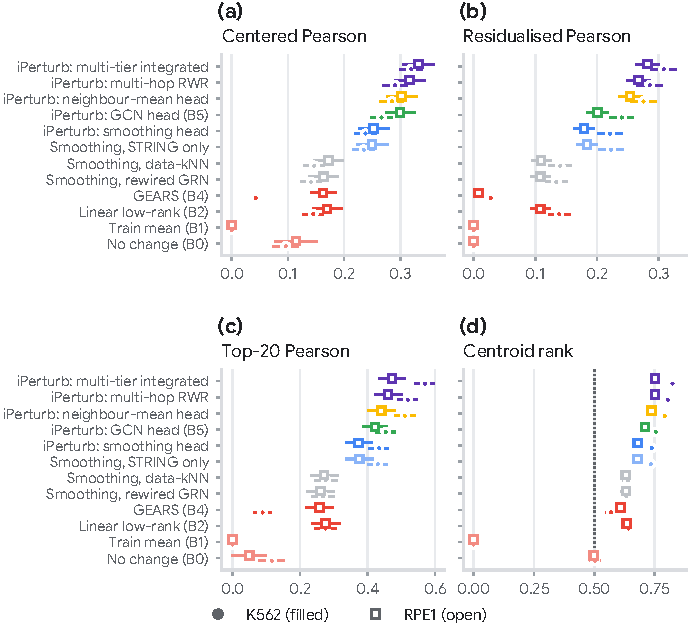
\includegraphics[width=\linewidth]{figures/fig3_generalization.pdf}
\caption{\textbf{iPerturb predicts responses to unseen CRISPRi targets in two human cell lines.}
Mean over held-out targets with 95\% bootstrap intervals over unique targets (three target-held-out folds; K562 $n=$ \datanum{k562_nuniq}, RPE1 $n=$ \datanum{rpe1_nuniq}). Filled circles, K562; open squares, RPE1.
\textbf{(a)}~Centred correlation $\rho_c$ (primary; the training mean scores 0 by construction).
\textbf{(b)}~Correlation after projecting the training-mean direction out of both profiles ($\rho_r$).
\textbf{(c)}~Top-20 centred correlation.
\textbf{(d)}~Mean normalised rank of the correct perturbation (centroid accuracy; 0.5 is chance).
Rewired-GRN and data-kNN graphs are controls with the same read-out and tuning grid.}
\label{fig:results}
\end{figure}

iPerturb, with multi-hop propagation integrated across evidence tiers, reaches $\rho_c=$ \datanum{g12_k562_prop_integrated__nnls} in K562 and \datanum{g12_rpe1_prop_integrated__nnls} in RPE1, a gain of \datanum{g12d_k562_int_b2} and \datanum{g12d_rpe1_int_b2} over the linear low-rank baseline.
The gain holds for every metric in Table~\ref{tab:main}, including the magnitude-free correlation $\rho_r$ and the centroid rank, so it reflects the shape of the response rather than its size.
iPerturb exceeds GEARS~\cite{roohani2024predicting} trained on the same folds ($\rho_c=$ \datanum{k562_gears_rc} and \datanum{rpe1_gears_rc}) and CPA and biolord with gene-ontology descriptions of unseen targets, which stay close to the mean response.
Released checkpoints of scGPT and STATE, whose pretraining overlaps with these screens, are listed for reference ($^\dagger$ in Table~\ref{tab:main}).

The gain comes from the GRN, not from the capacity of the read-out.
With the same read-out and tuning grid, the GRN improves on its degree-preserving rewired version by \datanum{k562_d_ip_rew_rc} (K562) and \datanum{rpe1_d_ip_rew_rc} (RPE1) and on a graph learned from the training responses alone by \datanum{k562_d_ip_knn_rc} and \datanum{rpe1_d_ip_knn_rc}\datanumif{g12rw_d_k562}{, and the integrated propagation improves on the same pipeline run over rewired tier graphs by \datanum{g12rw_d_k562} and \datanum{g12rw_d_rpe1}}; zeroing each training row's own-target entry leaves the gain unchanged (\datanum{k562_d_ip_noself_rc} and \datanum{rpe1_d_ip_noself_rc}; Table~\ref{tab:paired}).
Every read-out of the GRN improves on the linear baseline, from one-step smoothing of gene embeddings (\datanum{k562_d_ip_b2_rc} and \datanum{rpe1_d_ip_b2_rc}) to a graph convolutional network and the neighbour mean, and reading the graph over multiple hops adds a further \datanum{g12d_k562_rwr_one} (K562) and \datanum{g12d_rpe1_rwr_one} (RPE1) over one hop (Section~\ref{sec:ablation_tiers}).

\begin{table}[!t]
\centering
\caption{\textbf{iPerturb outperforms baselines and controls on held-out CRISPRi targets.} Unique-target means over three folds (bold: best per column among held-out models). $\rho_c$: centred correlation; $\rho_r$: after removing the training-mean direction; $\rho_{20}$: top-20 centred correlation; Cent.: mean normalised centroid rank; AUPRC: differentially expressed genes (|Welch $z|>4$). $^\dagger$Released pretrained checkpoint evaluated without retraining; its pretraining data overlap with these screens. CPA (B7) and biolord (B8) use the official packages with gene-ontology embeddings for unseen targets (Appendix~\ref{app:external}); external models are scored on the targets they support.}
\label{tab:main}
\scriptsize
\setlength{\tabcolsep}{1.5pt}
\begin{tabular}{lccccc}
\toprule
\multicolumn{6}{l}{\textbf{K562} (699 held-out targets)}\\
Model & $\rho_c$ & $\rho_r$ & $\rho_{20}$ & Cent. & AUPRC\\\midrule
No change (B0) & 0.096 & 0.000 & 0.116 & 0.503 & 0.099\\
Train mean (B1) & 0.000 & 0.000 & 0.000 & 0.000 & 0.031\\
Linear low-rank (B2) & 0.145 & 0.139 & 0.275 & 0.641 & 0.110\\
Smoothing, rewired GRN & 0.141 & 0.134 & 0.268 & 0.633 & 0.110\\
Smoothing, data-kNN graph & 0.147 & 0.141 & 0.277 & 0.640 & 0.112\\
Smoothing, STRING only & 0.235 & 0.223 & 0.430 & 0.735 & 0.132\\
iPerturb: smoothing head & 0.238 & 0.221 & 0.434 & 0.737 & 0.132\\
iPerturb: GCN head (B5) & 0.267 & 0.240 & 0.454 & 0.755 & 0.140\\
iPerturb: neighbour-mean head & \textbf{0.285} & \textbf{0.276} & \textbf{0.511} & \textbf{0.791} & \textbf{0.162}\\
\midrule
\multicolumn{6}{l}{\textbf{RPE1} (743 held-out targets)}\\
Model & $\rho_c$ & $\rho_r$ & $\rho_{20}$ & Cent. & AUPRC\\\midrule
No change (B0) & 0.115 & 0.000 & 0.050 & 0.498 & \textbf{0.245}\\
Train mean (B1) & 0.000 & 0.000 & 0.000 & 0.000 & 0.054\\
Linear low-rank (B2) & 0.170 & 0.108 & 0.276 & 0.634 & 0.175\\
Smoothing, rewired GRN & 0.163 & 0.108 & 0.260 & 0.631 & 0.174\\
Smoothing, data-kNN graph & 0.172 & 0.109 & 0.271 & 0.630 & 0.175\\
Smoothing, STRING only & 0.250 & 0.184 & 0.375 & 0.679 & 0.192\\
iPerturb: smoothing head & 0.252 & 0.179 & 0.374 & 0.680 & 0.191\\
iPerturb: GCN head (B5) & 0.299 & 0.201 & 0.422 & 0.711 & 0.191\\
iPerturb: neighbour-mean head & \textbf{0.302} & \textbf{0.254} & \textbf{0.440} & \textbf{0.737} & 0.204\\
\bottomrule
\end{tabular}
\end{table}

\subsection{The learnable Hill propagation is faithful to the Hill form and efficient as a matrix product}
\label{sec:results_hill}
\begin{figure}[!t]
\centering
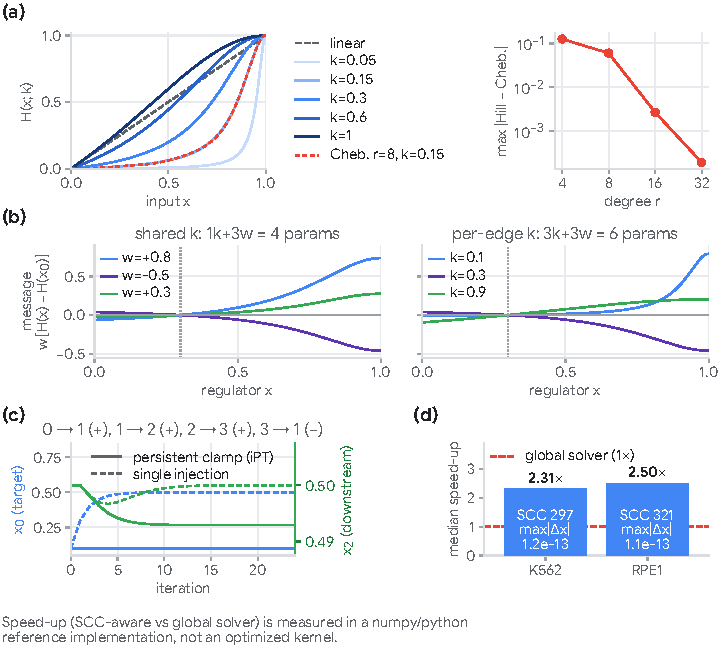
\includegraphics[width=\linewidth]{figures/fig2_operator.pdf}
\caption{\textbf{The regulatory operator of iPerturb.}
\textbf{(a)}~Modified Hill transfer functions of Eq.~\eqref{eq:hill} for five dissociation constants, the linear transfer, and the degree-8 Chebyshev form for $k=0.15$; the inset shows the maximal approximation error against the degree.
\textbf{(b)}~Messages of one regulator to three targets with a shared $k$ (rescaled copies of one shape) or edge-specific $k$ (three shapes).
\textbf{(c)}~A persistent clamp re-imposes the perturbed gene at every update, whereas a single injection lets it relax (four-gene motif with feedback; $x_2$ on the right axis).
\textbf{(d)}~Median speed-up of the SCC-aware solver over the global solver.}
\label{fig:operator}
\end{figure}
The Chebyshev form approximates the Hill curve to \datanum{cheb_err_r16} at degree 16 (worst case over $k\in[0.05,1]$; Figure~\ref{fig:operator}a).
Inside the full fixed-point iteration on the curated K562 network with heterogeneous regulator constants and 200 clamped targets, the equilibrium differs from exact Hill propagation by at most \datanum{eq_cheb16_spmm_dx} at degree 16, and sparse and dense products agree exactly.
The SCC-aware solver reproduces the global solver to \datanum{k562_scc_diff} with a median speed-up of \datanum{k562_scc_speed}$\times$ (K562) and \datanum{rpe1_scc_speed}$\times$ (RPE1; Figure~\ref{fig:operator}d).

Aggregating messages as a matrix product makes propagation efficient on dense evidence: on the 247k-edge association network (A100, batch 128, 24 damped updates) it reduces the step time from \datanum{bench_gpu_assoc_128_E0_ms}\,ms to \datanum{bench_gpu_assoc_128_E1_ms}\,ms and the peak memory from \datanum{bench_gpu_assoc_128_E0_mb}\,MB to \datanum{bench_gpu_assoc_128_E1_mb}\,MB, i.e.\ \datanum{speedratio_lo}- to \datanum{speedratio_hi}-fold faster with \datanum{memratio_lo}- to \datanum{memratio_hi}-fold less memory across batch sizes (Figure~\ref{fig:ablation}c).
The Chebyshev form extends this to edge-specific learnable shapes: edge-wise evaluation needs activations of size $B\times E\times r$ and exceeds the 40\,GB device at batch 128 with $r=16$, whereas the matrix form applies one sparse matrix with $Er$ non-zeros and fits in \datanum{pe_spmm_r16_128_gb}\,GB (\datanum{pe_memratio_r8_128}-fold less memory at $r=8$; outputs agree to \datanum{pe_equiv}; Figure~\ref{fig:ablation}d).

\subsection{iPerturb explains predictions by named neighbours and signed regulatory paths}
\label{sec:results_expl}
\begin{figure}[!t]
\centering
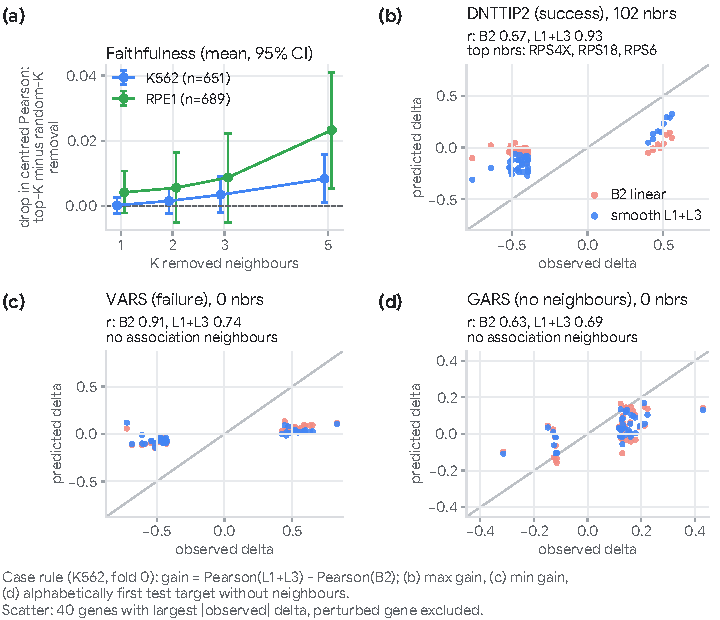
\includegraphics[width=\linewidth]{figures/fig5_explain.pdf}
\caption{\textbf{Neighbour explanations are faithful.}
\textbf{(a)}~Removing the top-$K$ attributed neighbours of a test target lowers its agreement with the observed profile more than removing $K$ random neighbours (mean difference with 95\% interval; targets with at least six neighbours).
\textbf{(b--d)}~Cases chosen by a rule fixed beforehand (K562 fold 0): largest gain over the linear baseline, smallest gain, and the first target without neighbours. Neighbours are association evidence, not causal paths.}
\label{fig:explain}
\end{figure}
Each prediction is attributed to the neighbours that support it, by the change in the prediction when a neighbour is removed, without access to the observed response.
Removing the five most attributed neighbours lowers the centred correlation with the observed profile more than removing five random neighbours, by \datanum{k562_faith5} in K562 (\datanum{k562_faith_n} targets) and \datanum{rpe1_faith5} in RPE1 (\datanum{rpe1_faith_n}; Figure~\ref{fig:explain}a).
The largest gain in the pre-specified K562 fold is DNTTIP2, a nucleolar protein whose three most attributed neighbours are the ribosomal proteins RPS4X, RPS18 and RPS6 (Figure~\ref{fig:explain}b).
Propagation recovers such functional modules more generally (Figure~\ref{fig:applications}): all 30 top-scoring neighbours of the held-out ribosomal gene RPL11 are ribosomal proteins, and predicted profiles of test perturbations cluster by gene family (86\% of edges between annotated genes join the same family, against 21\% by chance).

\begin{figure}[!t]
\centering
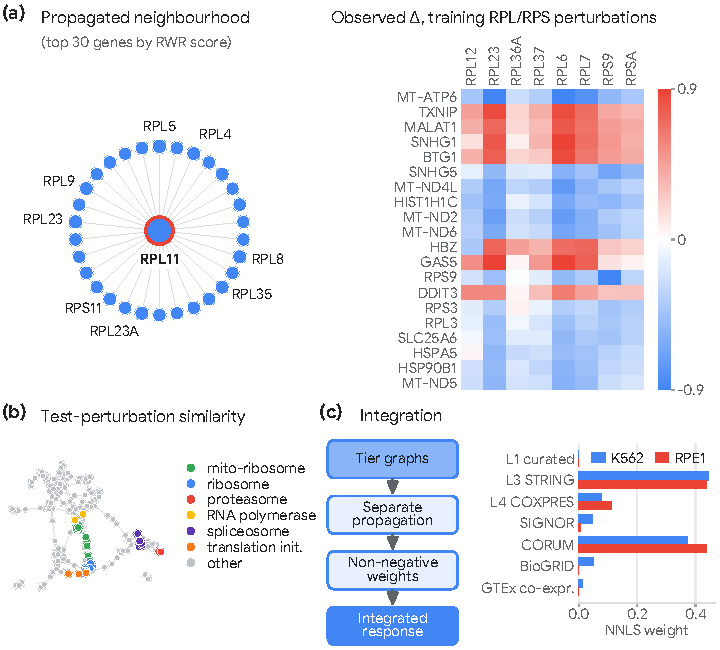
\includegraphics[width=\linewidth]{figures/fig_applications.pdf}
\caption{\textbf{Propagation over the association network recovers functional modules.}
\textbf{(a)}~Random-walk-with-restart neighbourhood of the held-out ribosomal gene RPL11 (K562, fold 0; node area proportional to propagation score) and the observed responses of eight training ribosomal perturbations, whose profiles correlate at 0.52 on average.
\textbf{(b)}~Test perturbations joined to their three most similar predicted profiles; edges between family-annotated nodes join the same family in 86.0\% of 43 cases against 21.1\% expected by chance.
\textbf{(c)}~Integration of tier-specific propagations with non-negative weights (mean over three folds); the protein-association tiers carry most of the weight.}
\label{fig:applications}
\end{figure}

On the regulatory side, we simulated CRISPRi as a persistent partial clamp on the signed network (Eq.~\eqref{eq:mech}) and compared the predicted direction with the measured response of held-out targets that have regulatory out-edges (\datanum{mech_k562_ntargets} K562 and \datanum{mech_rpe1_ntargets} RPE1 test perturbations; Figure~\ref{fig:mechanism}).
Among responding genes ($|z|>3$) one hop downstream, the signed paths predict the direction correctly for \datanum{mech_k562_real_h1}~\datanum{mech_k562_real_h1_ci} in K562 (\datanum{mech_k562_real_h1_n} genes) and \datanum{mech_rpe1_real_h1}~\datanum{mech_rpe1_real_h1_ci} in RPE1 (\datanum{mech_rpe1_real_h1_n} genes), above the same network with permuted signs (\datanum{mech_k562_signperm_h1} and \datanum{mech_rpe1_signperm_h1}) or rewired edges (\datanum{mech_k562_rewired_h1} and \datanum{mech_rpe1_rewired_h1}).
The controls lie above 0.5 because most responding genes move in the same direction after a knockdown, so the comparison isolates the information in the signs.
In the reported case, SSRP1 in K562 acts through MYC on ribosomal-protein genes along activating edges supported by CollecTRI and OmniPath, and the predicted down-regulation matches three of the five most responsive genes shown (Figure~\ref{fig:mechanism}c).
Signed paths longer than one hop are reported as candidate mechanisms with their supporting databases (Section~\ref{sec:ablation_hops}).

\begin{figure}[!t]
\centering
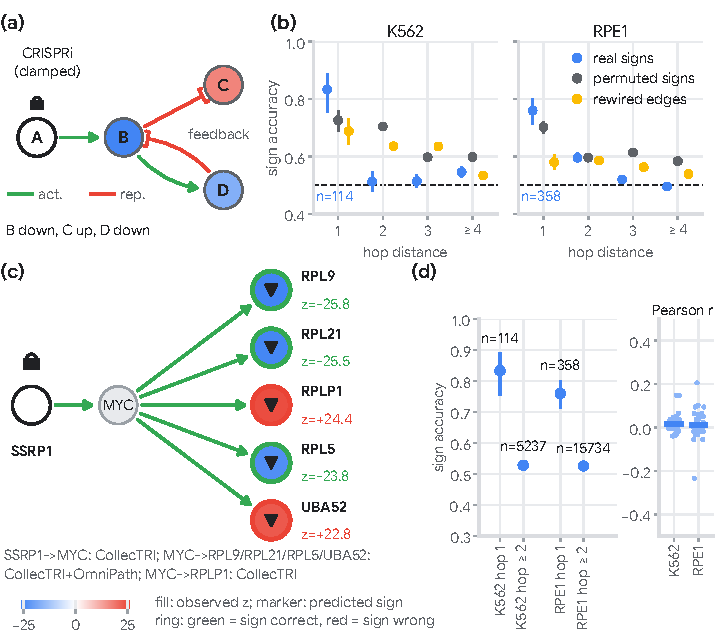
\includegraphics[width=\linewidth]{figures/fig_mechanism.pdf}
\caption{\textbf{Signed regulatory paths explain first-hop responses.}
\textbf{(a)}~A CRISPRi perturbation of A clamps A and lowers B, raises C (repressed by B) and lowers D, as computed by the model.
\textbf{(b)}~Sign accuracy of the predicted direction among responding genes ($|z|>3$) of held-out targets, by regulatory distance, for the real network and for controls with permuted edge signs or rewired edges (Wilson 95\% intervals, pooled over draws).
\textbf{(c)}~A mechanism report for one held-out K562 target: predicted sign (marker) against observed response (fill), supporting databases below.
\textbf{(d)}~Real-network accuracy at the first hop versus later hops, and the correlation between predicted and observed responses across reached genes.}
\label{fig:mechanism}
\end{figure}

\section{Ablation Study}
\label{sec:ablation}
We ablate the two components of iPerturb, the context-specific GRN (evidence layers, cell-line tier, further databases, propagation kernels) and the learnable Hill propagation (transfer function, certified variant, loss), and the preprocessing. All differences are paired over unique held-out targets with 95\% bootstrap intervals (Table~\ref{tab:paired}).

\subsection{Evidence layers and controls}
\label{sec:ablation_layers}
Figure~\ref{fig:ablation}b summarises the layers of the GRN and the controls of Section~\ref{sec:results_pred}: STRING alone, the curated tier plus STRING, a degree-preserving rewired version, a graph learned from the training data, and the real graph with own-target entries zeroed. Only the real association evidence changes $\rho_c$ relative to no graph; the curated tier adds nothing beyond STRING, and controls with the same capacity and tuning grid gain nothing.

\subsection{Evidence tiers and multi-hop propagation}
\label{sec:ablation_tiers}
\begin{table}[t]
\centering
\caption{\textbf{Each evidence tier as a propagation graph, and multi-hop read-outs.} Unique-target mean $\rho_c$ over three target-held-out folds; the response of a held-out target is the propagated, normalised response of training targets over the graph, with the restart probability (or the number of hops) chosen on validation targets.}
\label{tab:tiers}
\footnotesize
\begin{tabular}{lcc}
\toprule
Graph (random walk with restart, $\alpha$ selected) & K562 $\rho_c$ & RPE1 $\rho_c$\\\midrule
Linear low-rank (B2) & 0.145 & 0.170\\
L1 curated (CollecTRI/OmniPath/TRRUST) & 0.131 & 0.162\\
L1 + SIGNOR & 0.146 & 0.175\\
L3 STRING & 0.298 & 0.313\\
L3 CORUM complexes & 0.263 & 0.278\\
L3 BioGRID physical & 0.241 & 0.264\\
L4 COXPRESdb & 0.173 & 0.208\\
L4 GTEx co-expression & 0.170 & 0.195\\
L2 ChIP-Atlas (cell line) & 0.130 & --\\
L1+L3, one hop (neighbour mean) & 0.282 & 0.301\\
L1+L3, random walk with restart (multi-hop) & 0.291 & 0.316\\
L1+L3, truncated 2--3 hops & 0.299 & 0.321\\
All tiers, propagated separately and integrated & 0.319 & 0.333\\
\bottomrule
\end{tabular}
\end{table}
We replaced the smoothing head by propagation of the observed training responses over each tier alone (Table~\ref{tab:tiers}) in the manner of network propagation~\cite{cowen2017network}. Association evidence of protein-level tiers carries the signal: STRING alone reaches $\rho_c=$ \datanum{g12_k562_prop_L3__rwr} (K562) and \datanum{g12_rpe1_prop_L3__rwr} (RPE1), CORUM complexes and BioGRID interactions are weaker but informative, whereas the curated regulatory tier (L1) and co-expression tiers (L4) stay near the linear baseline (\datanum{g12_k562_B2_linear} and \datanum{g12_rpe1_B2_linear}). Adding signed SIGNOR edges to L1 changes $\rho_c$ by \datanum{g12d_k562_signor_l1} (K562) and \datanum{g12d_rpe1_signor_l1} (RPE1). CORUM and BioGRID are worse than STRING (\datanum{g12d_k562_corum_l3} and \datanum{g12d_k562_biogrid_l3} in K562), and GTEx co-expression does not improve on COXPRESdb. Reading the same L1+L3 graph beyond the first hop helps: random walks with restart improve on the one-hop neighbour mean by \datanum{g12d_k562_rwr_one} (K562) and \datanum{g12d_rpe1_rwr_one} (RPE1), and truncated two- to three-step walks by \datanum{g12d_k562_trunc_one} and \datanum{g12d_rpe1_trunc_one}. Finally, propagating each tier separately and combining the read-outs with non-negative weights fitted on validation targets gives a further \datanum{g12d_k562_int_rwr} (K562) and \datanum{g12d_rpe1_int_rwr} (RPE1) over L1+L3 with random walks, and \datanum{g12d_k562_int_b2} and \datanum{g12d_rpe1_int_b2} over the linear baseline. The weights concentrate on the protein-association tiers (K562: STRING \datanum{g12w_k562_L3}, CORUM \datanum{g12w_k562_corum}, BioGRID \datanum{g12w_k562_biogrid}, COXPRESdb \datanum{g12w_k562_L4}, GTEx co-expression \datanum{g12w_k562_gtex_coex}, curated L1 \datanum{g12w_k562_L1}; RPE1: STRING \datanum{g12w_rpe1_L3}, CORUM \datanum{g12w_rpe1_corum}), so multi-hop propagation adds measurable accuracy, while the curated regulatory tier contributes explanation rather than prediction. The ChIP-Atlas cell-line tier (L2) does not improve over the linear baseline either (Table~\ref{tab:tiers}).

\subsection{Cell-line-specific tier}
\label{sec:ablation_context}
\datanumif{g7_d_k_hep}{\emph{Does the cell-line-specific tier carry cell-line-specific predictive signal?} We tested this in K562, the only line with a non-empty tier, with the smoothing head of Section~\ref{sec:results_pred} and a criterion registered before the run: the K562 tier must beat both foreign-line tiers. It does not. Adding the K562 GeneHancer tier to the L1+L3 graph changes the centred correlation by \datanum{g7_d_k_base} relative to the base graph, by \datanum{g7_d_k_hep} relative to adding the HepG2 tier and by \datanum{g7_d_k_jur} relative to the Jurkat tier; the enlarged graph is better than its degree-preserving rewired version, which also scrambles L1+L3, by \datanum{g7_d_k_rew}. The cell-line-specific tier therefore differs strongly between lines but adds no measurable predictive gain over generic association evidence in this setting.}

\subsection{Hill versus linear propagation}
\label{sec:ablation_hill}
Following the pre-registered gate, we trained the shared-Hill model and a linear model with the same graph, decoder and budget as a residual on the linear baseline for the reachable targets (\datanum{k562_g2_reach_n} K562 and \datanum{rpe1_g2_reach_n} RPE1 unique targets over three folds). All differences in the centred correlation are below 0.002 in either direction. The Hill form relative to the linear form is \datanum{k562_g2_h2_b3} in K562 and \datanum{rpe1_g2_h2_b3} in RPE1 (marginally positive in RPE1), relative to the linear baseline without graph \datanum{k562_g2_h2_b2} and \datanum{rpe1_g2_h2_b2}, and the real graph relative to a rewired graph is \datanum{k562_g2_h2_rew} and \datanum{rpe1_g2_h2_rew}; the pre-registered criterion (an advantage over both the linear form and the no-graph baseline, and over the rewired graph) was not met. An oracle readout with its scale fitted on the test targets themselves added nothing, so the limit is the information in the signed core rather than the optimiser. The conclusion is unchanged for a certified, anti-vanishing variant (log-odds state so that large responses are not squashed, a leaky Hill transfer that keeps a gradient where the curve is flat, a contraction guaranteed for every parameter value, Appendix~\ref{app:convergence}) trained with a correlation-based loss that does not shrink with the size of the response: relative to no graph, the Hill form changes $\rho_c$ on reachable targets by \datanum{g10d_k562_gn2_hill4_mse} (MSE) and \datanum{g10d_k562_gn2_hill4_corr} (correlation loss) in K562 and by \datanum{g10d_rpe1_gn2_hill4_mse} and \datanum{g10d_rpe1_gn2_hill4_corr} in RPE1 (Table~\ref{tab:certhill}); every interval includes zero. The Hill-form operator is therefore a faithful and efficient implementation of the regulatory model, not a source of additional predictive accuracy on this data.

\begin{figure}[t]
\centering
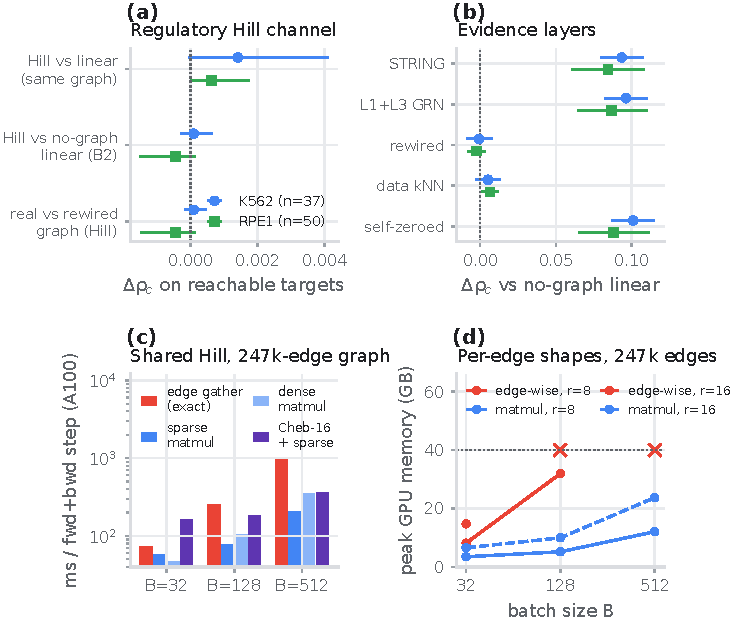
\includegraphics[width=\linewidth]{figures/fig4_ablation_efficiency.pdf}
\caption{\textbf{Ablations and efficiency.}
\textbf{(a)}~Hill-form versus linear propagation on the curated signed core, reachable test targets only (differences in $\rho_c$; \datanum{k562_g2_reach_n} K562 and \datanum{rpe1_g2_reach_n} RPE1 unique targets).
\textbf{(b)}~Change in $\rho_c$ relative to the no-graph linear model for evidence layers and controls (STRING only; L1+L3; rewired; graph learned from training data; L1+L3 with own-target entries zeroed).
\textbf{(c)}~Time per forward and backward step for the regulator-shared Hill operator on the 247k-edge association graph (A100).
\textbf{(d)}~Peak memory for edge-specific Chebyshev shapes (crosses: out of memory on 40\,GB).}
\label{fig:ablation}
\end{figure}

\subsection{Preprocessing}
\label{sec:ablation_prep}
Weighting training perturbations by cell number or by response precision did not help consistently (K562 \datanum{prep_k562_wn} and \datanum{prep_k562_wp} in $\rho_c$; RPE1 \datanum{prep_rpe1_wn} and \datanum{prep_rpe1_wp}), so the headline models are unweighted.

\section{Conclusion and Discussion}
\label{sec:discussion}

We introduced iPerturb, which builds a cell-line-specific regulatory network from five evidence tiers and propagates perturbations through it with a learnable transfer function that follows the Hill function, so that every prediction can be traced to named genes and edges. On held-out CRISPRi targets in K562 and RPE1 the tiered network carries predictive signal that matched rewired and data-derived graphs do not, multi-hop propagation of training responses over the tiers, integrated across tiers, is the strongest read-out (\datanum{g12_k562_prop_integrated__nnls} and \datanum{g12_rpe1_prop_integrated__nnls} in $\rho_c$ against \datanum{k562_b2_rc} and \datanum{rpe1_b2_rc} for the linear baseline), and the Hill-form operator reproduces exact Hill propagation to \datanum{eq_cheb16_spmm_dx} while its matrix-product form is memory-lean on dense graphs. Two limitations are central. First, the tiers that carry the predictive gain (curated regulation and protein association) are the same for every cell line; the cell-line-specific enhancer tier, testable only in K562, differs strongly between lines but did not improve prediction over a foreign line's tier or over the base graph, so its context specificity is descriptive rather than predictive in this setting. Second, on the curated signed core, which reaches only \datanum{k562_signed_out_pct}--\datanum{rpe1_signed_out_pct}\% of the perturbed genes in these essential-gene screens, a nonlinear Hill transfer does not predict better than a linear one, and the gain over a linear low-rank model comes from association evidence rather than from curated regulation. The mechanism-level test sharpens this: the signed network predicts the direction of direct regulatory effects, but the signed multi-hop cascade is not supported beyond the first hop in these endpoint data, so we present longer paths only as candidate mechanisms, and we prove only that the multi-hop quantity is well defined and has a unique convergence point (Appendix~\ref{app:convergence}), not that it is correct. We read the coverage limitation as a statement about the screens, not about biology: the screens perturb mostly non-TF genes, and a signed core cannot propagate what it does not reach.

Several limitations qualify these results. The predicted endpoint is the mean response, not a distribution of cells. RNA abundance is a proxy for regulator activity and endpoint data cannot identify time constants, so the fixed-point operator is a steady-state model; neighbour attributions are tested by ablation but are association paths, not validated mechanisms. The folds and seeds reuse the same biological screens, and graph and no-graph models were tuned on comparable but not identical budgets; matched controls share their grid. The largest gains are obtained for genes in well-characterised complexes (for example, ribosomal-protein neighbours), which are enriched in essential-gene screens, and the transfer to screens with few such complexes is untested. The GeneHancer tier is empty for RPE1, so the cell-line-specific tier is tested in K562 only; a test with the training-perturbation tier (Level 5) is left to future work. Future work will add more cell lines and a genome-wide screen with more transcription-factor targets, and test edge-specific learnable shapes, which the matrix-multiplication form now makes affordable, on data in which a signed core has more reach.

\section*{Conflict of interests, acknowledgments, funding, and data availability}
\textit{Conflict of Interests.} The authors declare that they have no competing interests.

\textit{Funding.} This work was supported by the AI Institute of Fulbright University Vietnam and Google.

\textit{Data and Software Availability.} The CRISPRi Perturb-seq datasets analysed in this study are publicly available from Replogle et al.~\cite{replogle2022mapping}. Prior biological knowledge was obtained from TRRUST, CollecTRI, OmniPath, GeneHancer v5.26, STRING v12 and COXPRESdb; GeneHancer is licence-gated and is not redistributed. The source code, the frozen pre-registration of the evaluation protocol with its later addenda, figure-generation scripts and the files from which every number in this paper is generated accompany the submission and will be released in the public iPerturb repository (\url{https://github.com/kagtgi/iPerturb}) at publication.


\bibliographystyle{splncs04}
\bibliography{references}
\appendix
\section{Additional protocol details}
\label{app:protocol}
\paragraph{Splits and fitting.} Three target-held-out folds per line (70/15/15\%, stratified by TF status, control-expression tertile and curated out-degree bin; seed 42, fold-specific seeds). The smoothing head selects $k\in\{5,10,20,40\}$ and $\alpha\in\{0,0.25,0.5,0.75\}$ on validation perturbations (selected settings: K562, \datanum{k562_cfg}; RPE1, \datanum{rpe1_cfg}); the ridge penalty is $10^{-2}$. The GCN has two layers, hidden size 64, residual self-weights, AdamW (learning rate $10^{-3}$ or $3\times10^{-3}$, weight decay $10^{-3}$), at most 200 epochs, patience 20, three seeds. Hill-form models use $n=2$, damping 0.5, 24 updates, learning rates $\{0.003,0.01\}$ and penalties $\{10^{-3},10^{-1}\}$ on the per-gene decoder offset, selected on validation reachable targets; the clamp strength $\zeta$ is the median training knockdown.
\paragraph{Pre-registration.} The evaluation protocol was written and hashed before any graph model was fitted. Later analyses (association smoothing, controls, GCN, explanations, context-specific tier, efficiency study, neighbour-free fallback) were added as dated addenda before they were run; the fallback analysis is exploratory and is not part of the headline numbers.
\paragraph{GEARS.} Trained with the official package on at most 100 cells per perturbation and 3,000 control cells (log1p of counts per $10^4$), for 6 epochs (fewer than the package default, which exceeded the memory of our 83\,GB host at the full cell count), hidden size 64, with its default gene-ontology graph; targets absent from its ontology set are excluded from its evaluation. Its predictions are expressed relative to its own control mean, whereas the observed responses use batch-matched controls, so GEARS is centred on the mean of its predictions for a sample of 300 training targets before scoring (the raw correlation is reported in the repository). These settings make GEARS a budget-limited baseline.

\section{Efficiency measurements}
\label{app:bench}
\begin{table}[!ht]
\centering
\caption{Time per forward and backward step (ms) and peak memory (MB) of the regulator-shared Hill operator (24 updates, A100 40\,GB). E0: exact Hill, edge gather/scatter; E1: exact Hill, sparse matrix product; E2: dense product; C1: degree-16 Chebyshev form, sparse product.}
\label{tab:bench}
\footnotesize
\begin{tabular}{llrrrr}
\toprule
Graph & Batch & E0 & E1 & E2 & C1\\\midrule
curated, 10k edges & 128 & 37 / 942 & 72 / 1054 & 104 / 1592 & 179 / 4001\\
curated, 10k edges & 512 & 73 / 3708 & 151 / 3315 & 346 / 3791 & 305 / 15018\\
\midrule
association, 247k edges & 128 & 250 / 6949 & 77 / 1078 & 103 / 1606 & 185 / 4025\\
association, 247k edges & 512 & 960 / 27689 & 208 / 3338 & 346 / 3803 & 360 / 15041\\
\bottomrule
\end{tabular}
\end{table}
On the CPU, the edge-wise form was the fastest for the sparse curated graph at every batch size (\datanum{bench_cpu_l1_128_E0_ms}\,ms at batch 128 against \datanum{bench_cpu_l1_128_E1_ms}\,ms for the sparse product), and on the association graph the dense product matched it (\datanum{bench_cpu_assoc_128_E2_ms}\,ms vs.\ \datanum{bench_cpu_assoc_128_E0_ms}\,ms).

\section{External baselines}
\label{app:external}
All external models were scored with the folds, metrics and centring of the other models (predictions are centred on the mean prediction for training targets). \emph{STATE}: the released State Transition checkpoints for Replogle-HVG data (zero-shot and few-shot variants, K562 and RPE1), evaluated without retraining; their pretraining data overlap with these screens (marked $^\dagger$). \emph{scGPT}: the whole-human checkpoint without fine-tuning; the official perturbation head is trained from scratch, so we ran a zero-shot in silico knockout (target expression set to zero in 100 control cells, change of the predicted expression averaged over cells) on the 1,199 most expressed in-vocabulary genes; targets outside the vocabulary or with near-zero control expression are excluded. \emph{biolord}: official package, with the gene-ontology neighbour vector of the GEARS gene-ontology graph as the attribute of the perturbed gene; no tuning. \emph{CPA}: \texttt{cpa-tools} with the same neighbour vectors as frozen perturbation embeddings, the hyper-parameters of its Norman tutorial, at most 50 cells per training target and a wall-clock cap of 25 minutes per fold (a reduced budget).

\section{Data replay}
\label{app:replay}
An independent re-computation of the target of ten random K562 perturbations directly from the raw counts (no chunking or sparse accumulation) reproduced the stored responses to within $4.5\times10^{-8}$ (single-precision rounding); the script and its output are in the repository.

\begin{table}[!ht]
\centering
\caption{\textbf{Certified, anti-vanishing Hill propagation on reachable held-out targets.} Unique-target mean $\rho_c$ and paired difference to the no-graph linear baseline (95\% bootstrap interval); all variants use the same graph, decoder, optimiser and tuning grid. Predictions are not numerically collapsed (standard deviation of the learned correction $10^{-3}$ against a residual standard deviation of about $0.06$--$0.09$), but they carry no usable signal.}
\label{tab:certhill}
\scriptsize
\begin{tabular}{lcccc}
\toprule
Reachable targets & K562 $\rho_c$ & $\Delta$ vs B2 & RPE1 $\rho_c$ & $\Delta$ vs B2\\\midrule
No graph (B2) & 0.073 & ref. & 0.147 & ref.\\
Linear propagation, MSE & 0.069 & -0.0041 [-0.0139, +0.0017] & 0.146 & -0.0012 [-0.0045, +0.0010]\\
Linear propagation, correlation loss & 0.067 & -0.0055 [-0.0161, +0.0018] & 0.145 & -0.0022 [-0.0051, -0.0001]\\
Certified Hill, MSE & 0.073 & +0.0001 [-0.0016, +0.0020] & 0.147 & -0.0003 [-0.0014, +0.0006]\\
Certified Hill, correlation loss & 0.070 & -0.0024 [-0.0086, +0.0016] & 0.146 & -0.0006 [-0.0026, +0.0010]\\
Certified Hill, correlation + Huber & 0.070 & -0.0024 [-0.0087, +0.0016] & 0.146 & -0.0006 [-0.0026, +0.0010]\\
\bottomrule
\end{tabular}
\end{table}

\section{Convergence of multi-hop propagation}
\label{app:convergence}
We show that the multi-hop propagation used by iPerturb has a unique convergence point (a fixed point) that is reached geometrically from any starting state, and that the hop-by-hop decomposition used for explanations is well defined. Throughout, $W\in\mathbb{R}^{G\times G}$ holds the signed effect of gene $j$ on gene $i$ ($W_{ij}$), $g$ is the clamped (perturbed) gene, $R$ the set of free genes, $\|W\|_\infty=\max_i\sum_j|W_{ij}|$ is the largest total incoming weight, $\rho(\cdot)$ the spectral radius and $|W|$ the entry-wise absolute value. Convergence is a property of the operator; it does not make a prediction correct (Remark~\ref{rem:notclaimed}).

\paragraph{Operators.} (O1)~\emph{linear:} $\Delta x_R=W_{RR}\Delta x_R+W_{Rg}\Delta x_g$. (O2/O3)~\emph{Hill-form:} with a state $z_R$ ($z=\mathrm{logit}\,x$; the sigmoid-state variant iterates $x$ directly), baseline $z^0$ and clamped $z_g$,
\begin{equation}
F_i(z)=z^0_i+\sum_{j}W_{ij}\big[T(\sigma(z_j))-T(\sigma(z^0_j))\big],\qquad T(x)=(1-\lambda)H(x;k_j)+\lambda x,
\label{eq:Fmap}
\end{equation}
iterated as $z^{t+1}=(1-\eta)z^t+\eta F(z^t)$ with the clamped coordinate held fixed at every step.

\begin{lemma}[Hill slope]\label{lem:hill}
For $n=2$ and $k\le\sqrt3$, $L_H(k):=\max_{x\in[0,1]}|H'(x;k)|=\dfrac{9(1+k^2)}{8\sqrt3\,k}$, attained at $1-x=k/\sqrt3$. With leak $\lambda$, $L_T\le(1-\lambda)L_H(k)+\lambda$.
\end{lemma}
\begin{proof}
With $u=1-x$, $H=k^2(1-u^2)/(u^2+k^2)$ and $|H'|=2u\,k^2(1+k^2)/(u^2+k^2)^2$. The derivative of $u/(u^2+k^2)^2$ has the sign of $k^2-3u^2$, so the maximum is at $u=k/\sqrt3\le1$, where $u^2+k^2=4k^2/3$ and $|H'|=9(1+k^2)/(8\sqrt3k)$. The leak adds slope $\lambda$ and removes at most $\lambda L_H$.
\end{proof}
Numerically $L_H=\datanum{lh_0p05}$ at $k=0.05$, $\datanum{lh_0p3}$ at $k=0.3$ and $\datanum{lh_1p0}$ at $k=1$; the formula agrees with a dense-grid maximum in the test suite.

\begin{proposition}[Existence]\label{prop:exist}
For every $W$, every parameter value and every clamp, the map~\eqref{eq:Fmap} has a fixed point.
\end{proposition}
\begin{proof}
$T$ takes values in $[0,1]$, so each bracket in~\eqref{eq:Fmap} lies in $[-1,1]$ and $F$ maps $\mathbb{R}^R$ into the compact convex box $\{|z_i-z_i^0|\le\|W\|_\infty\}$; $F$ is continuous, and Brouwer's theorem applies. (For the sigmoid state the box is $[0,1]^R$.)
\end{proof}

\begin{theorem}[Uniqueness and geometric convergence]\label{thm:contract}
Let $q:=\tfrac{L_T}{4}\|W_{RR}\|_\infty<1$ and $q_\eta:=1-\eta(1-q)$. Then the damped clamped iteration is a contraction of $(\mathbb{R}^R,\|\cdot\|_\infty)$ with constant $q_\eta$. It has a unique fixed point $z^\ast$, which is also the unique fixed point of $F$, and for every start $z^0$ and all $t$,
\[
\|z^t-z^\ast\|_\infty\le q_\eta^{\,t}\|z^0-z^\ast\|_\infty,\qquad \|z^t-z^\ast\|_\infty\le\frac{q_\eta}{1-q_\eta}\|z^t-z^{t-1}\|_\infty .
\]
A tolerance $\tau$ is reached after $t\ge\ln\!\big(\tau(1-q_\eta)/\|z^1-z^0\|_\infty\big)/\ln q_\eta$ steps.
\end{theorem}
\begin{proof}
Since $\sigma'\le1/4$ and $|T'|\le L_T$, $|F_i(z)-F_i(z')|\le\sum_j|W_{ij}|\,L_T\tfrac14|z_j-z'_j|$, hence $\|F(z)-F(z')\|_\infty\le q\|z-z'\|_\infty$ on the free coordinates (the clamped coordinate does not move). The damped map is the convex combination $(1-\eta)\mathrm{id}+\eta F$, with constant $1-\eta+\eta q=q_\eta$. Banach's fixed-point theorem gives existence, uniqueness and the first bound; the second follows from the triangle inequality $\|z^t-z^\ast\|\le\|z^t-z^{t+1}\|+q_\eta\|z^t-z^\ast\|$ and the bound on $\|z^{t+1}-z^t\|\le q_\eta\|z^t-z^{t-1}\|$.
\end{proof}
\begin{corollary}[Certified parametrisation]\label{cor:cert}
GraphNet2 sets $\|W\|_\infty=\gamma\,\sigma(\varrho)\,4/L_T(k)$ with $\gamma\le\tfrac12$ (incoming weights normalised to sum one, then scaled by a learnable gain through $\sigma(\varrho)$). Since $\|W_{RR}\|_\infty\le\|W\|_\infty$, $q\le\gamma\le\tfrac12$ for every value of $k\in[0.05,1]$ and of the learnable parameters, so Theorem~\ref{thm:contract} holds for every model the optimiser can reach. With $\eta=\tfrac12$, $q_\eta\le\tfrac34$.
\end{corollary}

\begin{theorem}[Multi-hop response is an absolutely convergent walk sum]\label{thm:neumann}
Assume $\rho(|W|)<1$ (enforced by the scaling in the construction of $W$). Then for every clamped gene $g$ and free set $R$: (i)~$\rho(|W_{RR}|)\le\rho(|W|)<1$, so $I-W_{RR}$ is invertible; (ii)~$\sum_{k\ge0}W_{RR}^{\,k}W_{Rg}\Delta x_g$ converges absolutely to $(I-W_{RR})^{-1}W_{Rg}\Delta x_g$, so the hop contributions $\Delta x^{(k)}=W_{RR}^{k-1}W_{Rg}\Delta x_g$ and the contributions of individual walks are well defined and may be summed in any order; (iii)~with $v=(I-|W|)^{-1}\mathbf 1\ge\mathbf 1$ and $q_v:=1-1/\max_iv_i<1$, truncating after $K$ hops leaves an error $\|\sum_{k>K}\Delta x^{(k)}\|_v\le\frac{q_v^{K}}{1-q_v}\|W_{Rg}\Delta x_g\|_v$, where $\|x\|_v=\max_i|x_i|/v_i$.
\end{theorem}
\begin{proof}
(i)~$|W_{RR}|$ is a principal block of $|W|$; for non-negative matrices the spectral radius is monotone under entry-wise domination and under taking principal blocks (Perron--Frobenius), and $\rho(W_{RR})\le\rho(|W_{RR}|)$. (ii)~$|W_{RR}^kb|\le|W_{RR}|^k|b|$ and $\sum_k|W_{RR}|^k$ converges when $\rho<1$; absolute convergence permits rearrangement (Fubini) into hops and into walks. (iii)~$(I-|W|)^{-1}=\sum_k|W|^k\ge I$ entry-wise, so $v\ge\mathbf 1$ and $|W|v=v-\mathbf 1\le(1-1/\max v)\,v$. For any $x$, $|W_{RR}x|\le|W_{RR}||x|\le\|x\|_v|W|v\le q_v\|x\|_vv$ on $R$, so $\|W_{RR}x\|_v\le q_v\|x\|_v$ and the tail of the geometric series follows.
\end{proof}
\begin{remark}[Why $\rho(|W|)$]
The signed spectral radius does not suffice: $W=\bigl(\begin{smallmatrix}1&1\\-1&-1\end{smallmatrix}\bigr)$ has $\rho(W)=0$, but the block $W_{RR}=(1)$ for $R=\{1\}$ has $\rho=1$ and $I-W_{RR}$ is singular. Nor is $\|W\|_\infty<1$ needed: on the curated graphs the total incoming weight is $\|W\|_\infty=\datanum{cert_k562_inf_scaled}$ (K562) and $\datanum{cert_rpe1_inf_scaled}$ (RPE1) after scaling to $\rho(|W|)=\datanum{cert_k562_rho_scaled}$, while $q_v=\datanum{cert_k562_qv}$ and $\datanum{cert_rpe1_qv}$.
\end{remark}

\begin{proposition}[SCC-aware execution]\label{prop:scc}
Under Theorem~\ref{thm:contract}, iterating the strongly connected components of the free graph in topological order (a single update for acyclic singletons, a local damped iteration for feedback components with already settled inputs) converges to the same unique fixed point as the global iteration; genes not reachable from $g$ stay at their baseline.
\end{proposition}
\begin{proof}
Each block map is a restriction of $F$ with the constant of a principal block ($\le q_\eta$), hence a contraction for fixed inputs. The block solutions, composed in topological order, satisfy every equation of the full system, and the fixed point is unique, so the two coincide. A gene without a path from $g$ has all parents either unreachable or at baseline, so $x^0_i$ solves its equation, and by uniqueness equals the fixed point.
\end{proof}

\begin{proposition}[Response-propagation kernels]\label{prop:kernel}
For the association graph let $W=AD^{-1}$ (column-stochastic) and $S_\alpha=\alpha(I-(1-\alpha)W)^{-1}$, $\alpha\in(0,1]$. The series $\sum_k((1-\alpha)W)^k$ converges geometrically with ratio $1-\alpha$, every column of $S_\alpha$ is a probability vector (non-negative, sum one), and the symmetric normalisation $D^{-1/2}AD^{-1/2}$ has spectrum in $[-1,1]$, so $\rho((1-\alpha)W_{\rm sym})\le1-\alpha$. The heat kernel $e^{-tL}$, $L=D-A$, exists for all $t\ge0$. The propagated prediction $\sum_jS_{pj}\Delta_j/\sum_jS_{pj}$ is a convex combination of training responses and therefore stays in their convex hull.
\end{proposition}
\begin{proof}
$\|(1-\alpha)W\|_1=1-\alpha<1$ because the columns of $W$ sum to one; the column sums of $S_\alpha$ are $\alpha\sum_k(1-\alpha)^k=1$; non-negativity follows from the series. $L$ is positive semi-definite, so $e^{-tL}$ is a contraction semigroup.
\end{proof}

\begin{remark}[What is not claimed]\label{rem:notclaimed}
Convergence is not correctness. Endpoint data do not identify dynamics, the fixed point is a steady-state description, and the multi-hop signs beyond one hop are at chance on held-out targets (Section~\ref{sec:results_mech}); the theorems guarantee that the quantity we explain is well defined, not that it matches biology.
\end{remark}

\begin{table}[!ht]
\centering
\caption{\textbf{Convergence certificates on the curated signed graphs} (all values generated from the run). Linear operator: $\rho(|W|)$ before scaling, scaled value, and Neumann terms needed for $10^{-6}$ (median/max over 40 clamped genes); $q_v$ and the largest ratio of observed truncation error to the bound of Theorem~\ref{thm:neumann}(iii) ($\le1$ confirms the bound). Certified Hill-form operator at extreme and default parameters: contraction constants, steps to $10^{-6}$ from four random starts, spread of the solutions and fixed-point residual.}
\label{tab:cert}
\scriptsize
\begin{tabular}{lcc}
\toprule
& K562 & RPE1\\\midrule
$\rho(|W|)$ raw $\to$ scaled & \datanum{cert_k562_rho_raw} $\to$ \datanum{cert_k562_rho_scaled} & \datanum{cert_rpe1_rho_raw} $\to$ \datanum{cert_rpe1_rho_scaled}\\
Neumann terms to $10^{-6}$ (median / max) & \datanum{cert_k562_terms_med} / \datanum{cert_k562_terms_max} & \datanum{cert_rpe1_terms_med} / \datanum{cert_rpe1_terms_max}\\
$q_v$; truncation-bound ratio & \datanum{cert_k562_qv}; \datanum{cert_k562_trunc_ratio} & \datanum{cert_rpe1_qv}; \datanum{cert_rpe1_trunc_ratio}\\
$q$ (max over parameters); $q_\eta$ & \datanum{cert_k562_q}; \datanum{cert_k562_qeta} & \datanum{cert_rpe1_q}; \datanum{cert_rpe1_qeta}\\
Steps to $10^{-6}$ (max) & \datanum{cert_k562_iters} & \datanum{cert_rpe1_iters}\\
Spread of solutions; residual & \datanum{cert_k562_spread}; \datanum{cert_k562_resid} & \datanum{cert_rpe1_spread}; \datanum{cert_rpe1_resid}\\
\bottomrule
\end{tabular}
\end{table}
The restart-walk kernels have column sums equal to one to within \datanum{cert_rwr_coldev} for $\alpha\in\{0.1,0.5,0.9\}$.

\end{document}
